\flushbottom




%%============================================================================
%%============================================================================
\chapter{Green Functions}




%%============================================================================
\section{Inhomogeneous Equations and Homogeneous Boundary Conditions}

Consider a linear differential equation on the domain $\Omega$
subject to homogeneous boundary conditions.
\begin{equation}
  \label{L[u(bfx)]=f(bfx)B[u(bfx)]=0}
  L[u(\mathbf{x})] = f(\mathbf{x}) \quad \mathrm{for}\ \mathbf{x} \in \Omega, \quad
  B[u(\mathbf{x})] = 0 \quad \mathrm{for}\ \mathbf{x} \in \partial \Omega
\end{equation}
For example, $L[u]$ might be
\[ 
L[u] = u_t - \kappa \Delta u, \quad \mathrm{or} \quad
L[u] = u_{t t} - c^2 \Delta u.
\]
and $B[u]$ might be $u = 0$, or $\nabla u \cdot \hat{n} = 0$.


If we find a Green function $G(\mathbf{x}; \mathbf{x}i)$ that satisfies
\[ 
L[G(\mathbf{x};\mathbf{x}i)] = \delta(\mathbf{x}-\mathbf{x}i), \quad 
B[G(\mathbf{x};\mathbf{x}i)] = 0
\]
then the solution to Equation~\ref{L[u(bfx)]=f(bfx)B[u(bfx)]=0} is
\[ 
u(\mathbf{x}) = \int_\Omega G(\mathbf{x};\mathbf{x}i) f(\mathbf{x}i)\,\dd \mathbf{x}i. 
\]
We verify that this solution satisfies the equation and boundary condition.
\begin{align*}
  L[u(\mathbf{x})]   &= \int_\Omega L[G(\mathbf{x};\mathbf{x}i)] f(\mathbf{x}i)\,\dd \mathbf{x}i \\
  &= \int_\Omega \delta(\mathbf{x}-\mathbf{x}i) f(\mathbf{x}i)\,\dd \mathbf{x}i \\
  &= f(\mathbf{x}) \\
  B[u(\mathbf{x})] &= \int_\Omega B[G(\mathbf{x};\mathbf{x}i)] f(\mathbf{x}i)\,\dd \mathbf{x}i \\
  &= \int_\Omega 0\,f(\mathbf{x}i)\,\dd \mathbf{x}i \\
  &= 0
\end{align*}








%%==============================================================================
\section{Homogeneous Equations and Inhomogeneous Boundary Conditions}


Consider a homogeneous linear differential equation on the domain $\Omega$
subject to inhomogeneous boundary conditions,
\begin{equation}
  \label{L[u(bfx)]=0B[u(bfx)]=h(bfx)}
  L[u(\mathbf{x})] = 0 \quad \mathrm{for}\ \mathbf{x} \in \Omega, \quad
  B[u(\mathbf{x})] = h(\mathbf{x}) \quad \mathrm{for}\ \mathbf{x} \in \partial \Omega.
\end{equation}



If we find a Green function $g(\mathbf{x}; \mathbf{x}i)$ that satisfies
\[ 
L[g(\mathbf{x};\mathbf{x}i)] = 0, \quad 
B[g(\mathbf{x};\mathbf{x}i)] = \delta(\mathbf{x}-\mathbf{x}i)
\]
then the solution to Equation~\ref{L[u(bfx)]=0B[u(bfx)]=h(bfx)} is
\[ 
u(\mathbf{x}) = \int_{\partial \Omega} g(\mathbf{x};\mathbf{x}i) h(\mathbf{x}i)\,\dd \mathbf{x}i. 
\]
We verify that this solution satisfies the equation and boundary condition.
\begin{align*}
  L[u(\mathbf{x})] &= \int_{\partial \Omega} L[g(\mathbf{x};\mathbf{x}i)] h(\mathbf{x}i)\,\dd \mathbf{x}i \\
  &= \int_{\partial \Omega} 0\, h(\mathbf{x}i)\,\dd \mathbf{x}i \\
  &= 0 \\
  B[u(\mathbf{x})] &= \int_{\partial \Omega} B[g(\mathbf{x};\mathbf{x}i)] h(\mathbf{x}i)\,\dd \mathbf{x}i \\
  &= \int_{\partial \Omega} \delta(\mathbf{x}-\mathbf{x}i) h(\mathbf{x}i)\,\dd \mathbf{x}i \\
  &= h(\mathbf{x})
\end{align*}






\begin{Example}
  Consider the Cauchy problem for the homogeneous heat equation.
  \begin{gather*}
    u_t = \kappa u_{x x}, \quad -\infty < x < \infty, \quad t > 0 \\
    u(x,0) = h(x), \quad u(\pm \infty, t) = 0 
  \end{gather*}
  We find a Green function that satisfies
  \begin{gather*}
    g_t = \kappa g_{x x}, \quad -\infty < x < \infty, \quad t > 0 \\
    g(x,0; \xi) = \delta(x-\xi), \quad g(\pm \infty, t; \xi) = 0.
  \end{gather*}
  Then we write the solution
  \[
  u(x,t) = \int_{-\infty}^\infty g(x, t;\xi) h(\xi) \,\dd \xi.
  \]

  To find the Green function for this problem, we apply a Fourier transform
  to the equation and boundary condition for $g$.
  \begin{gather*}
    \hat{g}_t = - \kappa \omega^2 \hat{g}, \quad
    \hat{g}(\omega, 0;\xi) = \mathcal{F}[\delta(x-\xi)] \\
    \hat{g}(\omega, t; \xi) 
    = \mathcal{F}[\delta(x-\xi)] \e^{-\kappa \omega^2 t} \\
    \hat{g}(\omega, t; \xi) = \mathcal{F}[\delta(x-\xi)]
    \mathcal{F}\left[\sqrt{\frac{\pi}{\kappa t}}
      \exp \left( - \frac{x^2}{4 \kappa t} \right) \right]
  \end{gather*}
  We invert using the convolution theorem.
  \begin{gather*}
    g(x, t; \xi) = \frac{1}{2\pi} \int_{-\infty}^\infty \delta(\psi-\xi)
    \sqrt{\frac{\pi}{\kappa t}} 
    \exp \left( - \frac{(x-\psi)^2}{4 \kappa t} \right) \,\dd \psi \\
    = \frac{1}{\sqrt{4 \pi \kappa t}} 
    \exp \left( - \frac{(x-\xi)^2}{4 \kappa t} \right)
    \intertext{The solution of the heat equation is}
    \boxed{
      u(x,t) = \frac{1}{\sqrt{4 \pi \kappa t}}
      \int_{-\infty}^\infty \exp \left( - \frac{(x-\xi)^2}{4 \kappa t} \right) 
      h(\xi) \,\dd \xi.
      }
  \end{gather*}
\end{Example}



%%==============================================================================
\section{Eigenfunction Expansions for Elliptic Equations}


Consider a Green function problem for an elliptic equation on a 
finite domain.
\begin{gather}
  \label{L[G]=delta(bfx-bfxi)}
  L[G] = \delta(\mathbf{x} - \mathbf{x}i), \quad \mathbf{x} \in \Omega \\
  \nonumber
  B[G] = 0, \quad \mathbf{x} \in \partial \Omega
\end{gather}
Let the set of functions $\{ \phi_{\mathbf{n}} \}$ be orthonormal and
complete on $\Omega$.  (Here $\mathbf{n}$ is the multi-index 
$\mathbf{n} = n_1, \ldots, n_d$.) 
\[
\int_\Omega \overline{ \phi_{\mathbf{n}}(\mathbf{x}) } \phi_{\mathbf{m}}(\mathbf{x}) \,\dd \mathbf{x} 
= \delta_{\mathbf{n} \mathbf{m}}
\]
In addition, let the $\phi_{\mathbf{n}}$ be 
eigenfunctions of $L$ subject to the homogeneous boundary 
conditions.
\[
L \left[ \phi_{\mathbf{n}} \right] = \lambda_{\mathbf{n}} \phi_{\mathbf{n}}, \quad
B \left[ \phi_{\mathbf{n}} \right] = 0
\]

We expand the Green function in the eigenfunctions.
\[
G = \sum_{\mathbf{n}} g_{\mathbf{n}} \phi_{\mathbf{n}}(\mathbf{x})
\]
Then we expand the Dirac Delta function.
\begin{gather*}
  \delta(\mathbf{x} - \mathbf{x}i) = \sum_{\mathbf{n}} d_{\mathbf{n}} \phi_{\mathbf{n}}(\mathbf{x}) \\
  d_{\mathbf{n}} = \int_\Omega \overline{ \phi_{\mathbf{n}}(\mathbf{x}) } 
  \delta(\mathbf{x} - \mathbf{x}i) \,\dd \mathbf{x} \\
  d_{\mathbf{n}} = \overline{ \phi_{\mathbf{n}}(\mathbf{x}i) } 
\end{gather*}
We substitute the series expansions for the Green function and
the Dirac Delta function into Equation~\ref{L[G]=delta(bfx-bfxi)}.
\[
\sum_{\mathbf{n}} g_{\mathbf{n}} \lambda_{\mathbf{n}} \phi_{\mathbf{n}}(\mathbf{x})
= \sum_{\mathbf{n}} \overline{ \phi_{\mathbf{n}}(\mathbf{x}i) } \phi_{\mathbf{n}}(\mathbf{x}) 
\]
We equate coefficients to solve for the $g_{\mathbf{n}}$ and hence
determine the Green function.
\begin{gather*}
  g_{\mathbf{n}} = \frac{ \overline{ \phi_{\mathbf{n}}(\mathbf{x}i) } }{ \lambda_{\mathbf{n}} } \\
  G(\mathbf{x}; \mathbf{x}i) 
  = \sum_{\mathbf{n}} \frac{ \overline{ \phi_{\mathbf{n}}(\mathbf{x}i) } \phi_{\mathbf{n}}(\mathbf{x}) }
  { \lambda_{\mathbf{n}} } 
\end{gather*}








\begin{Example}
  Consider the Green function for the reduced wave equation, 
  $\Delta u - k^2 u$ in the rectangle, $0 \leq x \leq a$, 
  $0 \leq y \leq b$, and vanishing on the sides.

  First we find the eigenfunctions of the operator
  $L = \Delta - k^2 = 0$.   Note that $\phi = X(x) Y(y)$ 
  is an eigenfunction of $L$ if $X$ is an eigenfunction of
  $\frac{\partial^2}{\partial x^2}$ and $Y$ is an eigenfunction of $\frac{\partial^2}{\partial y^2}$.
  Thus we consider the two regular Sturm-Liouville eigenvalue problems:
  \begin{gather*}
    X'' = \lambda X, \quad X(0) = X(a) = 0 \\
    Y'' = \lambda Y, \quad Y(0) = Y(b) = 0
  \end{gather*}
  This leads us to the eigenfunctions
  \[
  \phi_{m n} = \sin \left( \frac{m \pi x}{a} \right)
  \sin \left( \frac{n \pi y}{b} \right).
  \]
  We use the orthogonality relation
  \[
  \int_0^{2 \pi} \sin \left( \frac{m \pi x}{a} \right)
  \sin \left( \frac{n \pi x}{a} \right) \,\dd x 
  = \frac{a}{2} \delta_{m n}
  \]
  to make the eigenfunctions orthonormal.
  \[
  \phi_{m n} = \frac{2}{\sqrt{a b}} \sin \left( \frac{m \pi x}{a} \right)
  \sin \left( \frac{n \pi y}{b} \right), \quad
  m,n \in \mathbb{Z}^+
  \]
  The $\phi_{m n}$ are eigenfunctions of $L$.
  \[
  L \left[ \phi_{m n} \right] 
  = - \left( \left( \frac{m \pi}{a} \right)^2 
    + \left( \frac{n \pi}{b} \right)^2
    + k^2 \right) \phi_{m n}
  \]
  By expanding the Green function and the Dirac Delta function in 
  the $\phi_{m n}$ and substituting into the differential equation
  we obtain the solution.
  \begin{gather*}
    G = \sum_{m,n = 1}^\infty \frac{ \frac{2}{\sqrt{a b}} 
      \sin \left( \frac{m \pi \xi}{a} \right)
      \sin \left( \frac{n \pi \psi}{b} \right)
      \frac{2}{\sqrt{a b}} 
      \sin \left( \frac{m \pi x}{a} \right)
      \sin \left( \frac{n \pi y}{b} \right) }
    { - \left( \left( \frac{m \pi}{a} \right)^2 
        + \left( \frac{n \pi}{b} \right)^2
        + k^2 \right) } \\
    \boxed{
      G(x,y;\xi,\psi) = - 4 a b \sum_{m,n = 1}^\infty
      \frac{ \sin \left( \frac{m \pi x}{a} \right)
        \sin \left( \frac{m \pi \xi}{a} \right)
        \sin \left( \frac{n \pi y}{b} \right) 
        \sin \left( \frac{n \pi \psi}{b} \right) }
      { (m \pi b)^2 + (n \pi a)^2 + (k a b)^2 }
      }
  \end{gather*}
\end{Example}






\begin{Example}
  Consider the Green function for Laplace's equation, 
  $\Delta u = 0$ in the disk, $|r| < a$,
  and vanishing at $r = a$.

  First we find the eigenfunctions of the operator
  \[
  \Delta = \frac{\partial^2}{\partial r^2} + \frac{1}{r} \frac{\partial}{\partial r} 
  + \frac{1}{r^2} \frac{\partial^2}{\partial \theta^2}.
  \]
  We will look for eigenfunctions of the form
  $\phi = \Theta(\theta) R(r)$.  We choose the $\Theta$ to be 
  eigenfunctions of $\frac{\dd^2}{\dd \theta^2}$ subject to the periodic
  boundary conditions in $\theta$.
  \begin{gather*}
    \Theta'' = \lambda \Theta, \quad \Theta(0) = \Theta(2 \pi), \quad
    \Theta'(0) = \Theta'(2 \pi) \\
    \Theta_n = \e^{i n \theta}, \quad n \in \mathbb{Z}
  \end{gather*}
  We determine $R(r)$ by requiring that $\phi$ be an eigenfunction
  of $\Delta$.
  \begin{gather*}
    \Delta \phi = \lambda \phi \\
    (\Theta_n R)_{r r} + \frac{1}{r} (\Theta_n R)_r
    + \frac{1}{r^2} (\Theta_n R)_{\theta \theta} 
    = \lambda \Theta_n R \\
    \Theta_n R'' + \frac{1}{r} \Theta_n R' 
    + \frac{1}{r^2} (-n^2) \Theta_n R = \lambda \Theta R \\
    \intertext{For notational convenience, we denote
      $\lambda = - \mu^2$.}
    R'' + \frac{1}{r} R' + \left( \mu^2 - \frac{n^2}{r^2} \right) R = 0,
    \quad R(0)\ \mathrm{bounded}, \quad R(a) = 0
  \end{gather*}
  The general solution for $R$ is
  \[
  R = c_1 J_{n}(\mu r) + c_2 Y_{n}(\mu r).
  \]
  The left boundary condition demands that $c_2 =0$.  The right boundary
  condition determines the eigenvalues.
  \[
  R_{n m} = J_{n} \left( \frac{j_{n,m} r}{a} \right), \quad
  \mu_{n m} = \frac{j_{n,m}}{a}
  \]
  Here $j_{n,m}$ is the $m^{\mathrm{th}}$ positive root of $J_n$.
  This leads us to the eigenfunctions
  \[
  \phi_{n m} = \e^{i n \theta} J_{n} \left( \frac{j_{n,m} r}{a} \right)
  \]
  We use the orthogonality relations
  \begin{gather*}
    \int_0^{2 \pi}     \e^{-i m \theta} \e^{i n \theta} \,\dd \theta
    = 2 \pi \delta_{m n}, \\
    \int_0^1 r J_\nu(j_{\nu,m} r) J_\nu(j_{\nu,n} r) \,\dd r 
    = \frac{1}{2} \left( {J'}_\nu(j_{\nu,n}) \right)^2
    \delta_{m n}
  \end{gather*}
  to make the eigenfunctions orthonormal. 
  \[
  \phi_{n m} = \frac{1}{ \sqrt{\pi} a | {J'}_{n}(j_{n,m}) | }
  \e^{i n \theta} J_{n} \left( \frac{j_{n,m} r}{a} \right), \quad
  n \in \mathbb{Z}, \quad m \in \mathbb{Z}^+
  \]
  The $\phi_{n m}$ are eigenfunctions of $L$.
  \[
  \Delta \phi_{n m} = - \left( \frac{j_{n,m}}{a} \right)^2 \phi_{n m}
  \]
  By expanding the Green function and the Dirac Delta function in 
  the $\phi_{n m}$ and substituting into the differential equation
  we obtain the solution.
  \begin{gather*}
    G = \sum_{n = -\infty}^\infty \sum_{m = 1}^\infty \frac{ \frac{1}{ \sqrt{\pi} a | {J'}_{n}(j_{n,m}) | }
      \e^{-i n \vartheta} J_{n} \left( \frac{j_{n,m} \rho}{a} \right)
      \frac{1}{ \sqrt{\pi} a | {J'}_{n}(j_{n,m}) | }
      \e^{i n \theta} J_{n} \left( \frac{j_{n,m} r}{a} \right) }
    { - \left( \frac{j_{n,m}}{a} \right)^2 } \\
    \boxed{
      G(r,\theta; \rho,\vartheta) = - \sum_{n = -\infty}^\infty \sum_{m = 1}^\infty 
      \frac{1}{ \pi (j_{n,m} {J'}_{n}(j_{n,m}))^2 }
      \e^{i n (\theta - \vartheta)} 
      J_{n} \left( \frac{j_{n,m} \rho}{a} \right)
      J_{n} \left( \frac{j_{n,m} r}{a} \right)
      }
  \end{gather*}
\end{Example}









%%==============================================================================
\section{The Method of Images}





Consider Poisson's equation in the upper half plane.
\begin{gather*}
  \nabla^2 u = f(x,y), \quad -\infty < x < \infty,\quad y > 0 
  \\
  u(x,0) = 0, \quad u(x,y) \to 0\ \mathrm{as}\ x^2 + y^2 \to \infty
\end{gather*}
The associated Green function problem is
\begin{gather*}
  \nabla^2 G = \delta(x-\xi)\delta(y-\psi), \quad -\infty < x < \infty,\quad y > 0 
  \\
  G(x,0|\xi,\psi) = 0, \quad G(x,y|\xi,\psi) \to 0\ \mathrm{as}\ x^2 + y^2 \to \infty.
\end{gather*}

We will solve the Green function problem with the method of images.  
We expand the domain to include the lower half plane.  We place a negative 
image of the source in the lower half plane.  This will make the Green 
function odd about $y = 0$, i.e. $G(x,0|\xi,\psi) = 0$.
\begin{gather*}
  \nabla^2 G = \delta(x-\xi)\delta(y-\psi) - \delta(x-\xi)\delta(y+\psi), \quad -\infty < x < \infty,\quad y > 0 
  \\
  G(x,y|\xi,\psi) \to 0\ \mathrm{as}\ x^2 + y^2 \to \infty
\end{gather*}

Recall that the infinite space Green function which satisfies
$\Delta F = \delta(x - \xi) \delta(y - \psi)$ is 
\[
F(x,y|\xi,\psi) = \frac{1}{4\pi} \ln\left( (x-\xi)^2 + (y-\psi)^2 \right).
\]
We solve for $G$ by using the infinite space Green function.
\begin{align*}
  G
  &= F(x,y|\xi,\psi) - F(x,y|\xi,-\psi)
  \\
  &= \frac{1}{4\pi} \ln \left( (x-\xi)^2 + (y-\psi)^2 \right)
  - \frac{1}{4\pi}\ln \left( (x-\xi)^2 + (y+\psi)^2 \right) 
  \\
  &= \frac{1}{4\pi} \ln \left( \frac{(x-\xi)^2 + (y-\psi)^2}{(x-\xi)^2 + (y+\psi)^2} \right)
\end{align*}

We write the solution of Poisson's equation using the Green function.
\begin{gather*}
  u(x,y) = \int_0^\infty \int_{-\infty}^\infty G(x,y|\xi,\psi) f(\xi,\psi) \,\dd \xi \,\dd \psi
  \\
  \boxed{
    u(x,y) = \int_0^\infty \int_{-\infty}^\infty \frac{1}{4\pi} \ln \left( \frac{(x-\xi)^2 + (y-\psi)^2}
      {(x-\xi)^2 + (y+\psi)^2} \right) f(\xi,\psi) \,\dd \xi \,\dd \psi
    }
\end{gather*}









\raggedbottom
%%=============================================================================
\exercises{
\pagebreak
\flushbottom
\section{Exercises}











\begin{Exercise}
  Consider the Cauchy problem for the diffusion equation with a source.
  \[
  u_t - \kappa u_{x x} = s(x,t), \quad u(x,0) = f(x), \quad 
  u \to 0\ \mathrm{as}\ x \to \pm\infty
  \]
  Find the Green function for this problem and use it to determine the 
  solution.
\end{Exercise}








\begin{Exercise}
  Consider the 2-dimensional wave equation
  \[ 
  u_{t t} - c^2 (u_{x x} + u_{y y}) = 0.
  \]
  \begin{enumerate} 
  \item 
    Determine the fundamental solution for this equation. 
    (i.e. response to source at $t = \tau$, $\mathbf{x} = \boldsymbol{\xi}$). 
    You may find the following information useful about the Bessel function:
    \begin{gather*}
      J_0(x) = \frac{1}{\pi} \int_0^\pi \e^{\imath x \cos{\theta}} \,\dd \theta,
      \\
      \int_0^\infty J_0(a x) \sin(b x) \,\dd x = 
      \begin{cases}
        0, & 0 < b < a \\ 
        \frac{1}{\sqrt{b^2-a^2}}, & 0 < a < b 
      \end{cases}
    \end{gather*}
  \item 
    Use the ``method of descents'' to recover the 1-D fundamental solution.
  \end{enumerate}
\end{Exercise}









\begin{Exercise}
  Consider the linear wave equation
  \[ 
  u_{t t} = c^2 u_{x x}, 
  \]
  with constant $c$, on the infinite domain $-\infty < x < \infty$.
  \begin{enumerate} 
  \item 
    By using the Fourier transform 
    find the solution of $G_{t t} = c^2 G_{x x}$ subject to initial conditions 
    $G(x,0) = 0$, $G_t(x,0) = \delta(x-\xi)$. 
  \item 
    Now use this to find $u$ in the case where $c = 1$, $u(x,0) = 0$, and
    \[ 
    u_t(x,0) = 
    \begin{cases}
      0 &|x| > 1 \\
      1 - |x| &|x| < 1 
    \end{cases}
    \]
    Sketch the solution in $x$ for fixed times $t < 1$ and $t > 1$ 
    and also indicate on the $x,t$ ($t>0$) plane the regions of qualitatively 
    different behavior of $u$.
  \end{enumerate}
\end{Exercise}







\begin{Exercise}
  Consider a generalized Laplace equation with non-constant coefficients
  of the form:
  \[ 
  \nabla^2 u + \mathbf{A}(\mathbf{x}) \cdot \nabla u + h(\mathbf{x}) u = q(\mathbf{x}), 
  \]
  on a region $V$ with $u = 0$ on the boundary $S$. Suppose we find a 
  Green function which satisfies
  \[ 
  \nabla^2 G + \mathbf{A}(\mathbf{x}) \cdot \nabla G + h(\mathbf{x}) G = 
  \delta(\mathbf{x} - \boldsymbol{\xi}). 
  \]
  Use the divergence theorem to derive an appropriate generalized Green's
  identity and show that 
  \[ 
  u(\boldsymbol{\xi}) \neq \int _V G(\mathbf{x}|\boldsymbol{\xi}) q(\mathbf{x}) \,\dd 
  \mathbf{x}. 
  \]
  What equation should the Green function satisfy? Note: this equation is
  called the {\it adjoint} of the original partial differential equation. 
\end{Exercise}









\begin{Exercise}
  Consider Laplace's equation in the infinite three dimensional domain 
  with two sources of equal strength $C$, opposite sign and 
  separated by a distance $\epsilon$.  
  \[ 
  \nabla^2 u = C \delta(\mathbf{x} - \boldsymbol{\xi}_+) -  C \delta(\mathbf{x} - \boldsymbol{\xi}_-),
  \]
  where $\boldsymbol{\xi}_{\pm}=(\pm \frac{\epsilon}{2},0,0)$. 
  \begin{enumerate} 
  \item 
    Find the solution in terms of the fundamental solutions. 
  \item 
    Now consider the limit in which the distance between sources 
    goes to zero ($\epsilon \to 0$) and the strength increases in such
    a way that $C \epsilon = D$ remains fixed. Show that the solution can be
    written
    \[ 
    u= - \frac{D x}{4 \pi r^3},
    \]
    where $r = |\mathbf{x}|$. 
    This is called the response to a {\it dipole} located at the origin, with 
    strength D, and oriented in the positive $x$ direction. 
  \item  
    Show that in general the response to a unit ($D = 1$) dipole at an
    arbitrary point $\boldsymbol{\xi}_0$ and oriented in the direction 
    of the unit vector $\mathbf{a}$ is
    \[ 
    u(\mathbf{x}) = - \frac{1}{4 \pi} \nabla_{\boldsymbol{\xi}} \left. 
      \left( \frac{1}{|\mathbf{x} - \boldsymbol{\xi}|} \right) 
    \right|_{\boldsymbol{\xi}=\boldsymbol{\xi}_0} \cdot \vec{a}
    \]
  \end{enumerate}
\end{Exercise}










\begin{Exercise}
  Consider Laplace's equation
  \[ 
  \nabla^2 u = 0,
  \]
  inside the unit circle with boundary condition $u = f(\theta)$. By using
  the Green function for the Dirichlet problem on the circle:
  \[ 
  G(\mathbf{x}|\boldsymbol{\xi}) = \frac{1}{2 \pi} 
  \ln \left( \frac{|\mathbf{x}-\boldsymbol{\xi}|}
    {|\boldsymbol{\xi}| |\mathbf{x} - \boldsymbol{\xi}^*|} \right),
  \]
  where $\boldsymbol{\xi}$ and $\boldsymbol{\xi}^*$ have the same polar angle and 
  $|\boldsymbol{\xi}^*|=\frac{1}{|\boldsymbol{\xi}|}$, show that the
  solution may be expressed in polar coordinates as 
  \[ 
  u(r, \theta) = \frac{1 - r^2}{2 \pi} 
  \int_0^{2 \pi} \frac{ f(\vartheta) }{ 1 + r^2 - 2 r \cos(\theta - \vartheta) } \,\dd \vartheta.
  \]
\end{Exercise}









\begin{Exercise}
  Consider an alternate derivation of the fundamental solution 
  of Laplace's equation 
  \[ 
  \nabla^2 u = \delta (\mathbf{x}),
  \]
  with $u\to 0$ as $|\mathbf{x}| \to \infty$ in three dimensions. 
  \begin{enumerate} 
  \item 
    Convert this equation to spherical coordinates. 
    You may define a new delta function
    \[ 
    \delta_3(r)=\delta(x)\delta(y)\delta(z) 
    \quad \mathrm{such that} \quad
    \int_B \delta_3(r) \,\dd V 
    = \begin{cases}
      1 & \mathrm{if B contains the origin} \\ 
      0 & \mathrm{otherwise} 
    \end{cases}
    \]
  \item 
    Show, by symmetry, that this can be reduced to an ordinary differential
    equation. Solve 
    to find the general solution of the homogeneous equation. Now
    determine the constants by using the constraint that $u \to 0$ 
    as $|\mathbf{x}| \to \infty$, and by integrating the partial differential equation
    over a small ball around the origin (and using Gauss' theorem). 
  \item 
    Now use similar ideas to re-derive the fundamental solution in 
    two dimensions. Can we still say $u \to 0$ as $|\mathbf{x}| \to \infty$?
    Use instead the constraint that $u = 0$ when $|\mathbf{x}| = 1$.
  \item 
    Finally derive the 2-D solution from the 3-D one using the 
    ``method of descent''. Consider Laplace's equation in three dimensions 
    with a line source at $x = 0$, $y = 0$, $-\infty < z < \infty$,
    \[  
    u_{xx} + u_{yy} + u_{zz} = \delta(x) \delta(y).
    \]
    Use the fundamental solution to find $u(r)$ 
    where $r = \sqrt{x^2 + y^2}$, and without loss of generality we have taken 
    the plane at $z = 0$. Then evaluate this integral to find $u$. 
    ({\it {Hint}}: first try to compute $u_r$) 
  \end{enumerate}
\end{Exercise}










\begin{Exercise}
  Consider the heat equation on the bounded domain $0 < x < L$ with fixed
  temperature at each end. Use Laplace transforms to determine 
  the Green Function which satisfies
  \begin{gather*}
    G_t - \nu G_{xx} = \delta(x-\xi) \delta(t), 
    \\
    G(0,t) = 0 \quad G(L,t) = 0,
    \\
    G(x,0^-) = 0.
  \end{gather*}
  
  \begin{enumerate} 
  \item 
    First show that 
    \[ 
    \mathcal{L}[G(x,t)] = \frac{  
      \cosh \left( \sqrt{ \frac{s}{\nu} } (L - x_> + x_<) \right)
      - \cosh \left( \sqrt{ \frac{s}{\nu} } (L - x_> - x_<) \right) }
    { 2 \sqrt{\nu s} \sinh \left( \sqrt{ \frac{s}{\nu} } L \right) }
    \]
    
  \item 
    Show that this can be re-written as 
    \[ 
    \mathcal{L}[G(x,t)] = \sum_{k=-\infty}^{\infty} \frac{1}{2 \sqrt{\nu s}} \e^{- \sqrt{\frac{s}{\nu}}|x-\xi-2kL|} 
    - \frac{1}{2 \sqrt{\nu s}} \e^{- \sqrt{\frac{s}{\nu}}|x+\xi-2kL|}.
    \]

  \item 
    Use this to find $G$ in terms of fundamental solutions
    \[  
    f(x,t) = \frac{1}{2 \sqrt{\nu \pi t}} \e^{-\frac{x^2}{4 \nu t}} ,
    \]
    and comment on how this Green's function corresponds to ``real'' and 
    ``image'' sources. Additionally compare this to the alternative 
    expression,
    \[ 
    G(x,t) = \frac{2}{L} \sum_{n=1}^{\infty} \e^{-\frac{\nu n^2 \pi^2}{L^2} t} 
    \sin{\frac{n \pi x}{L}} \sin{\frac{n \pi \xi}{L}},
    \]
    and comment on the convergence of the respective formulations for small 
    and large time. 
  \end{enumerate} 
\end{Exercise}










\begin{Exercise}
  Consider the Green function for the 1-D heat equation 
  \[ 
  G_t - \nu G_{xx} = \delta(x-\xi) \delta(t-\tau), 
  \]
  on the semi-infinite domain with insulated end
  \[ 
  G_x(0,t) = 0, \quad G \to 0\ \mathrm{as}\ x \to \infty,
  \] 
  and subject to the initial condition
  \[ 
  G(x,\tau^-)=0 .
  \]

  \begin{enumerate} 
  \item 
    Solve for $G$ with the Fourier cosine transform.
  \item 
    (15 points) Relate this to the fundamental solution on the infinite domain, 
    and discuss in terms of responses to ``real'' and ``image'' sources. 
    Give the solution for $x > 0$ of
    \begin{gather*}
      u_t - \nu u_{xx} = q(x,t), 
      \\
      u_x(0,t) = 0, \quad u \to 0\ \mathrm{as}\ x \to \infty,
      \\
      u(x,0) = f(x).
    \end{gather*}
  \end{enumerate}
\end{Exercise}












\begin{Exercise}
  Consider the heat equation
  \[ 
  u_t = \nu u_{x x} + \delta(x-\xi) \delta(t), 
  \]
  on the infinite domain $-\infty < x < \infty$, where we assume $u \to 0$ as
  $x \to \pm \infty$ and initially $u(x,0^-) = 0$. 

  \begin{enumerate}
  \item 
    First convert this to a problem where there is no forcing, so that 
    \[ 
    u_t = \nu u_{x x} 
    \]
    with an appropriately modified initial condition. 
  \item 
    Now use Laplace tranforms to convert this to an ordinary differential 
    equation in $\hat{u}(x,s)$, where
    $\hat{u}(x,s) = \mathcal{L}[u(x,t)]$. Solve this ordinary differential 
    equation and show that
    \[ 
    \hat{u}(x,s) = \frac{1}{2 \sqrt{\nu s}}e^{-\sqrt{\frac{s}{\nu}}|x-\xi|} .
    \]
    Recall $\hat{f}(s) = \mathcal{L}[f(t)] = \int_0^\infty \e^{-st} f(t)\,\dd t$.
  \item
    Finally use the Laplace inversion formula and Cauchy's Theorem on 
    an appropriate contour to compute $u(x,t)$. Recall 
    \[ 
    f(t) = \mathcal{L}^{-1}[F(s)] = \frac{1}{\imath 2 \pi} \int_\Gamma F(s) \e^{s t}\,\dd s,
    \]
    where $\Gamma$ is the Bromwich contour ($s = a + \imath t$ where $t \in (-\infty \ldots \infty)$ and 
    $a$ is a non-negative constant such that the contour lies to the 
    right of all poles of $\hat{f}$). 
  \end{enumerate}
\end{Exercise}







%% Green function for 1D wave equation on (-\infty..\infty).
\begin{Exercise}
  \label{wave_eqn_causal_green_fcn}
  Derive the causal Green function for the one dimensional wave equation on 
  $(-\infty..\infty)$.  That is, solve
  \begin{gather*}
    G_{t t} - c^2 G_{x x} = \delta(x - \xi) \delta(t - \tau), 
    \\
    G(x,t;\xi,\tau) = 0 \quad \mathrm{for}\ t < \tau.
  \end{gather*}
  Use the Green function to find the solution of the following wave equation 
  with a source term.
  \[
  u_{t t} - c^2 u_{x x} = q(x,t), \quad u(x,0) = u_t(x,0) = 0
  \]
\end{Exercise}





%%By reducing the problem to a series of one dimensional Green function
\begin{Exercise}
  By reducing the problem to a series of one dimensional Green function
  problems, determine $G(\mathbf{x}, \mathbf{x}i)$ if
  \[
  \nabla^2  G = \delta(\mathbf{x}-\mathbf{x}i)
  \]
  \begin{enumerate}
    \renewcommand{\labelenumi}{(\alph{enumi})}
    %%
  \item on the rectangle $0 < x < L$, $ 0 < y < H$ and
    \[
    G(0,y;\xi,\psi) = G_x(L,y;\xi,\psi) = G_y(x,0;\xi,\psi) = G_y(x,H;\xi,\psi) = 0
    \]
  \item on the box $0 < x < L$, $0 < y < H$, $0 < z < W$ with $G=0$
    on the boundary.
  \item on the semi-circle $0 < r < a$, $0 < \theta < \pi$ with $G=0$ on the
    boundary.
  \item on the quarter-circle $0 < r < a$, $0 < \theta < \pi/2$ with $G=0$ on
    the straight sides and  $G_r = 0$ at $r = a$.
  \end{enumerate}
\end{Exercise}






%% multi-dimensional eigenfunction.  \nabla^2  G = \delta(\mathbf{x}-\mathbf{x}_0)
\begin{Exercise}
  Using the method of multi-dimensional
  eigenfunction expansions, determine $G( \mathbf{x}, \mathbf{x}_0)$ if
  \[
  \nabla^2  G = \delta(\mathbf{x}-\mathbf{x}_0)
  \]
  and
  \begin{enumerate}
    \renewcommand{\labelenumi}{(\alph{enumi})}
    %%
  \item on the rectangle $(0<x<L,~0<y<H)$
    \[
    \begin{array}{rrrr}
      \mbox{at $x = 0$}, & \quad G = 0& \qquad \mbox{at $y = 0$}, &
      \quad {\displaystyle \frac{\partial G}{\partial y} = 0} \\
      \\
      \mbox{at $x = L$}, & \quad {\displaystyle \frac{\partial
          G}{\partial x} = 0}& \qquad \mbox{at $y = H$}, &
      \quad {\displaystyle \frac{\partial G}{\partial y}} = 0
    \end{array}
    \]
  \item on the rectangular shaped box $(0<x<L,~0<y<H,~0<z<W)$ with $G=0$
    on the six sides.
  \item on the semi-circle $(0<r<a,~0<\theta<\pi)$ with $G=0$ on the
    entire boundary.
  \item on the quarter-circle $(0<r<a,~0<\theta<\pi/2)$ with $G=0$ on
    the straight sides and  $\partial G / \partial r = 0$ at $r = a$.
  \end{enumerate}
\end{Exercise}








%% Using the method of images solve \nabla^2 G = \delta (\mathbf{x} - \mathbf{x}_0)
\begin{Exercise}
  Using the method of images solve
  \[
  \nabla^2 G = \delta (\mathbf{x} - \mathbf{x}_0)
  \]
  in the first quadrant  $(x \geq 0\ \mathrm{and}\ y \geq 0)$ 
  with $G=0$ at $x = 0$
  and $\partial G / \partial y = 0$ at $y = 0$. Use the Green function
  to solve in the first quadrant
  \begin{align*}
    \nabla^2 u & = 0 \\
    u(0,y) & =  g(y) \\
    \frac{\partial u}{\partial y}(x,0) &= h(x).
  \end{align*}
\end{Exercise}








%% Consider the wave equation defined on the half-line $x>0$:
\begin{Exercise}
  Consider the wave equation defined on the half-line $x>0$:
  \begin{align*}
    \frac{\partial^2 u}{\partial t^2} &= c^2 \frac{\partial^2 u}{\partial x^2} + Q(x,t), \\
    u(x,0) &= f(x) \\
    \frac{\partial u}{\partial t} (x,0) &= g(x)  \\
    u(0,t) &= h(t)
  \end{align*}
  \begin{enumerate}
    \renewcommand{\labelenumi}{(\alph{enumi})}
    %%
  \item Determine the appropriate Green's function using the method of images.
    %%
  \item Solve for $u(x,t)$ if $Q(x,t) = 0$, $f(x) = 0$, and $g(x) = 0$.
    %%
  \item For what values of $t$ does $h(t)$ influence $u(x_1, t_1)$. 
    Interpret this result physically.
  \end{enumerate}
\end{Exercise}






%% Green function for 1D wave equation. Initial conditions.
\begin{Exercise}
  \label{wave_eqn_IC_green_fcn}
  Derive the Green functions for the one dimensional wave equation on 
  $(-\infty..\infty)$ for non-homogeneous initial conditions. 
  Solve the two problems
  \begin{gather*}
    g_{t t} - c^2 g_{x x} = 0, \quad
    g(x,0;\xi,\tau) = \delta(x - \xi), \quad 
    g_t(x,0;\xi,\tau) = 0, \\
    \gamma_{t t} - c^2 \gamma_{x x} = 0, \quad
    \gamma(x,0;\xi,\tau) = 0, \quad 
    \gamma_t(x,0;\xi,\tau) = \delta(x - \xi),
  \end{gather*}
  using the Fourier transform.
\end{Exercise}


%% 1D wave equation on (-\infty..\infty) using Green functions.
\begin{Exercise}
  Use the Green functions from Problem~\ref{wave_eqn_causal_green_fcn}
  and Problem~\ref{wave_eqn_IC_green_fcn} to solve
  \begin{gather*}
    u_{t t} - c^2 u_{x x} = f(x,t), \quad x > 0, \quad -\infty < t < \infty \\
    u(x,0) = p(x), \quad u_t(x,0) = q(x).
  \end{gather*}
  Use the solution to determine the domain of dependence of the solution.
\end{Exercise}



%% Green function in a rectangle.
\begin{Exercise}
  Show that the Green function for the reduced wave equation, 
  $\Delta u - k^2 u = 0$ in the rectangle, $0 \leq x \leq a$, 
  $0 \leq y \leq b$, and vanishing on the sides is:
  \[
  G(x,y;\xi,\psi) = \frac{2}{a} \sum_{n = 1}^\infty 
  \frac{ \sinh(\sigma_n y_<) \sinh(\sigma_n(y_>-b)) }
  { \sigma_n \sinh(\sigma_n b) }
  \sin \left( \frac{n \pi x}{a} \right)
  \sin \left( \frac{n \pi \xi}{a} \right),
  \]
  where 
  \[
  \sigma_n = \sqrt{ k^2 + \frac{n^2 \pi^2}{a^2} }.
  \]
\end{Exercise}



%% Green function in quarter plane with mixed boundary conditions.
\begin{Exercise}
  Find the Green function for the reduced wave equation $\Delta u - k^2 u = 0$,
  in the quarter plane: $0 < x < \infty$, $0 < y < \infty$ subject to
  the mixed boundary conditions:
  \[
  u(x,0) = 0, \quad u_x(0,y) = 0.
  \]
  Find two distinct integral representations for $G(x,y;\xi,\psi)$.
\end{Exercise}





%% Green function on infinite sector.
\begin{Exercise}
  Show that in polar coordinates the Green function for $\Delta u = 0$ in
  the infinite sector, $0 < \theta < \alpha$, $0 < r < \infty$, and
  vanishing on the sides is given by,
  \[
  G(r, \theta, \rho, \vartheta ) = \frac{1}{4\pi} \ln \left(
    \frac{ \cosh \left( \frac{\pi}{\alpha} \ln \frac{r}{\rho} \right)
      - \cos \left( \frac{\pi}{\alpha} (\theta - \vartheta) \right) }
    { \cosh \left( \frac{\pi}{\alpha} \ln \frac{r}{\rho} \right)
      - \cos \left( \frac{\pi}{\alpha} (\theta + \vartheta) \right) }\right).
  \]
  Use this to find the harmonic function $u(r, \theta)$ in the given sector
  which takes on the boundary values:
  \[
  u(r,\theta) = u(r,\alpha) =
  \begin{cases}
    0 &\mathrm{for}\ r < c \\
    1 &\mathrm{for}\ r > c.
  \end{cases}
  \]
\end{Exercise}







%% Heat equation, method of images
\begin{Exercise}
  The Green function for the initial value problem,
  \[
  u_t - \kappa u_{x x} = 0, \quad u(x,0) = f(x),
  \]
  on $-\infty < x < \infty$ is
  \[
  G(x,t;\xi) = \frac{1}{\sqrt{4 \pi \kappa t}} \e^{-(x-\xi)^2 / (4 \kappa t)}.
  \]
  Use the method of images to find the corresponding Green function for the 
  mixed initial-boundary problems:
  \begin{enumerate}
  \item
    $\displaystyle u_t = \kappa u_{x x}, \quad u(x,0) = f(x)\ \mathrm{for}\
    x > 0, \quad u(0,t) = 0$,
  \item
    $\displaystyle u_t = \kappa u_{x x}, \quad u(x,0) = f(x)\ \mathrm{for}\
    x > 0, \quad u_x(0,t) = 0$.
  \end{enumerate}
\end{Exercise}










%% Green function for 1D wave equation on 0..L.
\begin{Exercise}
  Find the Green function (expansion) for the one dimensional wave equation
  $u_{t t} - c^2 u_{x x} = 0$ on the interval $0 < x < L$, subject to the
  boundary conditions:
  \begin{alignat*}{2}
    &\mathrm{a)} &\quad &u(0, t) = u_x(L, t) = 0, \\
    &\mathrm{b)} &\quad &u_x(0, t) = u_x(L, t) = 0. 
  \end{alignat*}
  Write the final forms in terms showing the propagation properties of the 
  wave equation, i.e., with arguments $((x \pm \xi) \pm (t - \tau))$.
\end{Exercise}



%% 1D wave equation on 0..1 with prescribed initial conditions.
\begin{Exercise}
  Solve, using the above determined Green function,
  \begin{gather*}
    u_{t t} - c^2 u_{x x} = 0, \quad 0 < x < 1, \quad t > 0, \\
    u_x(0, t) = u_x(1, t) = 0, \\
    u(x, 0) = x^2 (1 - x)^2, \quad u_t(x, 0) = 1.
  \end{gather*}
  For $c = 1$, find $u(x, t)$ at $x = 3/4$, $t = 7/2$.
\end{Exercise}










\raggedbottom
}
%%=============================================================================
\hints{
\pagebreak
\flushbottom
\section{Hints}






\begin{Hint}
  %% CONTINUE
\end{Hint}





\begin{Hint}
  %% CONTINUE
\end{Hint}






\begin{Hint}
  %% CONTINUE
\end{Hint}






\begin{Hint}
  %% CONTINUE
\end{Hint}






\begin{Hint}
  %% CONTINUE
\end{Hint}






\begin{Hint}
  %% CONTINUE
\end{Hint}







\begin{Hint}
  %% CONTINUE
\end{Hint}







\begin{Hint}
  %% CONTINUE
\end{Hint}







\begin{Hint}
  %% CONTINUE
\end{Hint}








\begin{Hint}
  %% CONTINUE
\end{Hint}





%% Green function for 1D wave equation. Initial conditions.
\begin{Hint}
  %% CONTINUE
\end{Hint}



%% Green function for 1D wave equation on (-\infty..\infty).
\begin{Hint}
  Take a Fourier transform in $x$.  This will give you an ordinary differential 
  equation Green function problem for $\hat{G}$.  Find the continuity and 
  jump conditions at $t = \tau$.  After solving for $\hat{G}$, do the 
  inverse transform with the aid of a table.
\end{Hint}



%% multi-dimensional eigenfunction.  \nabla^2  G = \delta(\mathbf{x}-\mathbf{x}_0)
\begin{Hint}
  %% CONTINUE
\end{Hint}






%% Using the method of images solve \nabla^2 G = \delta (\mathbf{x} - \mathbf{x}_0)
\begin{Hint}
  %% CONTINUE
\end{Hint}







%% Consider the wave equation defined on the half-line $x>0$:
\begin{Hint}
  %% CONTINUE
\end{Hint}






%% 1D wave equation on (-\infty..\infty) using Green functions.
\begin{Hint}
  %% CONTINUE
\end{Hint}





%% Green function in a rectangle.
\begin{Hint}
  %% CONTINUE
\end{Hint}



%% Green function in quarter plane with mixed boundary conditions.
\begin{Hint}
  Use Fourier sine and cosine transforms.
\end{Hint}





%% Green function on infinite sector.
\begin{Hint}
  The the conformal mapping $z = w^{\pi/\alpha}$ to map the sector to the 
  upper half plane.  The new problem will be
  \begin{align*}
    &G_{x x} + G_{y y} = \delta(x - \xi) \delta(y - \psi), 
    \quad -\infty < x < \infty, \quad 0 < y < \infty, \\
    &G(x,0,\xi,\psi) = 0, \\
    &G(x,y,\xi,\psi) \to 0\ \mathrm{as}\ x,y \to \infty.
  \end{align*}
  Solve this problem with the image method.
\end{Hint}






%% Heat equation, method of images
\begin{Hint}
  %% CONTINUE
\end{Hint}





%% Green function for 1D wave equation on 0..L.
\begin{Hint}
  %% CONTINUE
\end{Hint}




%% 1D wave equation on 0..1 with prescribed initial conditions.
\begin{Hint}
  %% CONTINUE
\end{Hint}






\raggedbottom
}
%%=============================================================================
\solutions{
\pagebreak
\flushbottom
\section{Solutions}










\begin{Solution}
  The Green function problem is 
  \[
  G_t - \kappa G_{x x} = \delta(x-\xi) \delta(t-\tau), \quad G(x,t|\xi,\tau) = 0\ \mathrm{for}\ t < \tau, \quad 
  G \to 0\ \mathrm{as}\ x \to \pm \infty
  \]
  We take the Fourier transform of the differential equation.
  \[
  \hat{G}_t + \kappa \omega^2 \hat{G} = \mathcal{F}[\delta(x-\xi)] \delta(t-\tau), \quad 
  \hat{G}(\omega,t|\xi,\tau) = 0\ \mathrm{for}\ t < \tau
  \]
  Now we have an ordinary differential equation Green function problem for 
  $\hat{G}$. The homogeneous solution of the ordinary differential equation is
  \[
  \e^{-\kappa \omega^2 t}
  \]
  The jump condition is
  \[
  \hat{G}(\omega,0;\xi,\tau^+) = \mathcal{F}[\delta(x - \xi)].
  \]
  We write the solution for $\hat{G}$ and invert using the convolution theorem.
  \begin{gather*}
    \hat{G} = \mathcal{F}[\delta(x - \xi)] \e^{- \kappa \omega^2 (t-\tau)} H(t-\tau)
    \\
    \hat{G} = \mathcal{F}[\delta(x - \xi)] 
    \mathcal{F} \left[ \sqrt{ \frac{\pi}{\kappa(t-\tau)} } \e^{-x^2 / (4 \kappa (t-\tau))} \right]
    H(t-\tau)
    \\
    G = \frac{1}{2 \pi} \int_{-\infty}^\infty \delta(x - y - \xi) \sqrt{ \frac{\pi}{\kappa(t-\tau)} } 
    \e^{-y^2 / (4 \kappa (t-\tau))} \,\dd y H(t - \tau)
    \\
    \boxed{
      G = \frac{1}{\sqrt{ 4 \pi \kappa(t-\tau) }} \e^{-(x-\xi)^2 / (4 \kappa (t-\tau))} H(t - \tau)
      }
  \end{gather*}
  We write the solution of the diffusion equation using the Green function.
  \begin{gather*}
    u = \int_0^\infty \int_{-\infty}^\infty G(x,t|\xi,\tau) s(\xi,\tau) \,\dd \xi \,\dd \tau
    + \int_{-\infty}^\infty G(x,t|\xi,0) f(\xi) \,\dd \xi
    \\
    \boxed{
      u = \int_0^t \frac{1}{\sqrt{4 \pi \kappa(t-\tau)}} \int_{-\infty}^\infty \e^{-(x-\xi)^2 / (4 \kappa (t-\tau))} s(\xi,\tau) 
      \,\dd \xi \,\dd \tau 
      + \frac{1}{\sqrt{4 \pi \kappa t}} \int_{-\infty}^\infty  \e^{-(x-\xi)^2 / (4 \kappa t)} f(\xi) \,\dd \xi
      }
  \end{gather*}
\end{Solution}








\begin{Solution}
  \begin{enumerate}
  \item
    We apply Fourier transforms in $x$ and $y$ to the Green function problem.
    \begin{gather*}
      G_{t t} - c^2 (G_{x x} + G_{y y}) = \delta(t - \tau) \delta(x - \xi) \delta(y - \eta)
      \\
      \hat{\hat{G}}_{t t} + c^2 \left( \alpha^2 + \beta^2 \right) \hat{\hat{G}} 
      = \delta(t - \tau) \frac{1}{2 \pi} \e^{-\imath \alpha \xi} \frac{1}{2 \pi} \e^{-\imath \beta \eta}
    \end{gather*}
    This gives us an ordinary differential equation Green function problem
    for $\hat{\hat{G}}(\alpha, \beta, t)$.        We find the causal solution.  That is, 
    the solution that satisfies $\hat{\hat{G}}(\alpha, \beta, t) = 0$ for $t < \tau$.
    \[
    \hat{\hat{G}} = \frac{ \sin \left( \sqrt{\alpha^2 + \beta^2} c (t - \tau) \right) }
    { c \sqrt{\alpha^2 + \beta^2} } \frac{1}{4 \pi^2} \e^{-\imath (\alpha \xi + \beta \eta)} H(t - \tau)
    \]
    Now we take inverse Fourier transforms in $\alpha$ and $\beta$.
    \[
    G = \int_{-\infty}^\infty \int_{-\infty}^\infty \frac{ \e^{\imath (\alpha (x - \xi) + \beta (y - \eta))}        }
    { 4 \pi^2 c \sqrt{\alpha^2 + \beta^2} } \sin \left( \sqrt{\alpha^2 + \beta^2} c (t - \tau) \right) 
    \,\dd \alpha \,\dd \beta H(t - \tau)
    \]
    We make the change of variables $\alpha = \rho \cos \phi$, $\beta = \rho \sin \phi$ and do the 
    integration in polar coordinates.
    \[
    G = \frac{1}{4 \pi^2 c} \int_0^{2 \pi} \int_0^\infty \frac{ \e^{\imath \rho ((x - \xi) \cos \phi + (y - \eta) \sin \phi)}  }
    { \rho } \sin \left( \rho c (t - \tau) \right) \rho \,\dd \rho \,\dd \phi H(t - \tau)
    \]
    Next we introduce polar coordinates for $x$ and $y$.
    \begin{gather*}
      x - \xi = r \cos \theta, \quad y - \eta = r \sin \theta
      \\
      G = \frac{1}{4 \pi^2 c} \int_0^\infty \int_0^{2 \pi} \e^{\imath r \rho (\cos \theta \cos \phi + \sin \theta \sin \phi)} \,\dd \phi
      \sin \left( \rho c (t - \tau) \right) \,\dd \rho H(t - \tau)
      \\
      G = \frac{1}{4 \pi^2 c} \int_0^\infty \int_0^{2 \pi} \e^{\imath r \rho \cos(\phi-\theta)} \,\dd \phi
      \sin \left( \rho c (t - \tau) \right) \,\dd \rho H(t - \tau)
      \\
      G = \frac{1}{2 \pi c} \int_0^\infty J_0(r \rho) \sin \left( \rho c (t - \tau) \right) \,\dd \rho 
      H(t - \tau)
      \\
      G = \frac{1}{2 \pi c} \frac{1}{\sqrt{ (c (t - \tau))^2 - r^2 } } H( c(t - \tau) - r )
      H(t - \tau)
      \\
      \boxed{
        G( \mathbf{x}, t | \boldsymbol{\xi}, \tau ) 
        = \frac{H( c(t - \tau) - | \mathbf{x} - \boldsymbol{\xi}| )}
        {2 \pi c \sqrt{ (c (t - \tau))^2 - | \mathbf{x} - \boldsymbol{\xi}|^2 } } 
        }
    \end{gather*}

  \item
    To find the 1D Green function, we consider a line source, 
    $\delta(x) \delta(t)$.  Without loss of generality, we have taken the source to 
    be at $x = 0$, $t = 0$.  We use the 2D Green function and integrate over
    space and time.
    \begin{gather*}
      g_{t t} - c^2 \Delta g = \delta(x) \delta(t)
      \\
      g = \int_{-\infty}^\infty \int_{-\infty}^\infty \int_{-\infty}^\infty 
      \frac{ H \left( c(t - \tau) - \sqrt{ (x - \xi)^2 + (y - \eta)^2 } \right) }
      {2 \pi c \sqrt{ (c (t - \tau))^2 - (x - \xi)^2 - (y - \eta)^2 } } \delta(\xi) \delta(\tau) 
      \,\dd \xi \,\dd \eta \,\dd \tau
      \\
      g = \frac{1}{2 \pi c} \int_{-\infty}^\infty
      \frac{ H \left( c t - \sqrt{ x^2 + \eta^2 } \right) }
      {\sqrt{ (c t)^2 - x^2 - \eta^2 } }\, \dd \eta
      \\
      g = \frac{1}{2 \pi c} \int_{- \sqrt{(c t)^2 - x^2}}^{\sqrt{(c t)^2 - x^2}}
      \frac{ 1 }{ \sqrt{ (c t)^2 - x^2 - \eta^2 } }\, \dd \eta
      H \left( c t - |x| \right)
      \\
      g(x,t|0,0) = \frac{1}{2 c} H \left( c t - |x| \right)
      \\
      \boxed{
        g(x,t|\xi,\tau) = \frac{1}{2 c} H \left( c (t - \tau) - |x - \xi| \right)
        }
    \end{gather*}
    
  \end{enumerate}
\end{Solution}







\begin{Solution}
  \begin{enumerate} 
  \item 
    \begin{gather*}
      G_{t t} = c^2 G_{x x}, \quad G(x,0) = 0, \quad G_t(x,0) = \delta(x-\xi)
      \\
      \hat{G}_{t t} = - c^2 \omega^2 \hat{G}, \quad \hat{G}(\omega,0) = 0, 
      \quad \hat{G}_t(\omega,0) = \mathcal{F}[\delta(x-\xi)]
      \\
      \hat{G} = \mathcal{F}[\delta(x-\xi)] \frac{1}{c \omega} \sin(c \omega t)
      \\
      \hat{G} = \frac{\pi}{c} \mathcal{F}[\delta(x-\xi)] \mathcal{F}[H(c t - |x|)]
      \\
      G(x,t) = \frac{\pi}{c} \frac{1}{2 \pi} \int_{-\infty}^\infty \delta(x-\xi-\eta) H(c t - |\eta|) \,\dd \eta
      \\
      G(x,t) = \frac{1}{2 c} H(c t - |x - \xi|)
    \end{gather*}
  \item 
    We can write the solution of 
    \[
    u_{t t} = c^2 u_{x x}, \quad u(x,0) = 0, \quad u_t(x,0) = f(x)
    \]
    in terms of the Green function we found in the previous part.
    \[
    u = \int_{-\infty}^\infty G(x,t|\xi) f(\xi) \,\dd \xi
    \]
    We consider $c = 1$ with the initial condition 
    $f(x) = (1 - |x|) H(1 - |x|)$.
    \[
    u(x,t) = \frac{1}{2} \int_{x-t}^{x+t} (1 - |\xi|) H(1 - |\xi|) \,\dd \xi
    \]
    First we consider the case $t < 1/2$.  We will use fact that the solution 
    is symmetric in $x$.
    \begin{gather*}
      u(x,t) = \begin{cases}
        0, &x+t < -1
        \\
        \frac{1}{2} \int_{-1}^{x+t} (1 - |\xi|) \,\dd \xi, &x-t < -1 < x+t
        \\
        \frac{1}{2} \int_{x-t}^{x+t} (1 - |\xi|) \,\dd \xi, &-1 < x-t,\ x+t < 1
        \\
        \frac{1}{2} \int_{x-t}^{1} (1 - |\xi|) \,\dd \xi, &x-t < 1 < x+t
        \\
        0, &1 < x-t
      \end{cases}
      \\
      u(x,t) = \begin{cases}
        0, &x+t < -1
        \\
        \frac{1}{4} (1 + t + x)^2 &x-t < -1 < x+t
        \\
        (1+x) t &-1 < x-t,\  x+t < 0
        \\
        \frac{1}{2} (2 t - t^2 - x^2) &x-t < 0 < x+t
        \\
        (1-x) t &0 < x-t,\  x+t < 1
        \\
        \frac{1}{4} (1 + t - x)^2 &x-t < 1 < x+t
        \\
        0, &1 < x-t
      \end{cases}
    \end{gather*}


    Next we consider the case $1/2 < t < 1$.
    \begin{gather*}
      u(x,t) = \begin{cases}
        0, &x+t < -1
        \\
        \frac{1}{2} \int_{-1}^{x+t} (1 - |\xi|) \,\dd \xi, &x-t < -1 < x+t
        \\
        \frac{1}{2} \int_{x-t}^{x+t} (1 - |\xi|) \,\dd \xi, &-1 < x-t,\ x+t < 1
        \\
        \frac{1}{2} \int_{x-t}^{1} (1 - |\xi|) \,\dd \xi, &x-t < 1 < x+t
        \\
        0, &1 < x-t
      \end{cases}
      \\
      u(x,t) = \begin{cases}
        0, &x+t < -1
        \\
        \frac{1}{4} (1 + t + x)^2 &-1 < x+t < 0
        \\
        \frac{1}{4} ( 1 - t^2 + 2 t (1 - x) + x(2 - x) ) &x-t < -1,\  0 < x+t
        \\
        \frac{1}{2} (2 t - t^2 - x^2) &-1 < x-t,\ x+t < 1
        \\
        \frac{1}{4} ( 1 - t^2 + 2 t (1 + x) - x(2 + x) ) &x-t < 0,\  1 < x+t
        \\
        \frac{1}{4} (1 + t - x)^2 &0 < x-t < 1
        \\
        0, &1 < x-t
      \end{cases}
    \end{gather*}


    Finally we consider the case $1 < t$.
    \begin{gather*}
      u(x,t) = \begin{cases}
        0, &x+t < -1
        \\
        \frac{1}{2} \int_{-1}^{x+t} (1 - |\xi|) \,\dd \xi, &-1 < x+t < 1
        \\
        \frac{1}{2} \int_{-1}^{1} (1 - |\xi|) \,\dd \xi, &x-t < -1,\ 1 < x+t
        \\
        \frac{1}{2} \int_{x-t}^{1} (1 - |\xi|) \,\dd \xi, &-1 < x-t < 1
        \\
        0, &1 < x-t
      \end{cases}
      \\
      u(x,t) = \begin{cases}
        0, &x+t < -1
        \\
        \frac{1}{4} (1 + t + x)^2 &-1 < x+t < 0
        \\
        \frac{1}{4} ( 1 - ( t + x - 2 )( t + x ) ) &0 < x+t < 1
        \\
        \frac{1}{2} &x-t < -1,\ 1 < x+t
        \\
        \frac{1}{4} ( 1 - ( t - x - 2 )( t - x ) ) &-1 < x-t < 0
        \\
        \frac{1}{4} (1 + t - x)^2 &0 < x-t < 1
        \\
        0, &1 < x-t
      \end{cases}
    \end{gather*}



    Figure~\ref{ut12t2} shows the solution at $t = 1/2$ and $t = 2$.
    \begin{figure}[h!]
      \begin{center}
        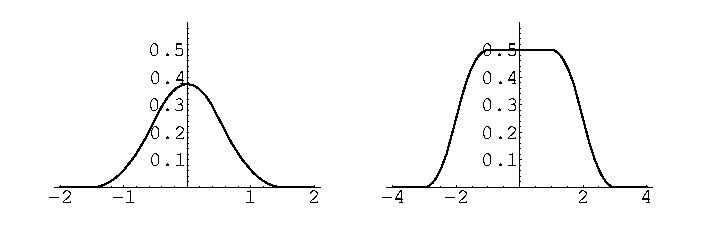
\includegraphics[width=0.75\textwidth]{pde/green/ut12t2}
      \end{center}
      \caption{The solution at two times.}
      \label{ut12t2}
    \end{figure}

    Figure~\ref{phaseplaneutf} shows the behavior of the solution 
    in the phase plane.  There are lines emanating form $x = -1,0,1$ showing
    the range of influence of these points.
    \begin{figure}[h!]
      \begin{center}
        \includegraphics[width=0.5\textwidth]{pde/green/phaseplaneutf}
      \end{center}
      \caption{The behavior of the solution in the phase plane.}
      \label{phaseplaneutf}
    \end{figure}
  \end{enumerate}
\end{Solution}









\begin{Solution}
  We define
  \[
  L[u] \equiv \nabla^2 u + \mathbf{a}(\mathbf{x}) \cdot \nabla u + h(\mathbf{x}) u.
  \]
  We use the Divergence Theorem to derive a generalized Green's Theorem.
  \begin{gather*}
    \int_V u L[v] \,\dd \mathbf{x}
    = \int_V u ( \nabla^2 v + \mathbf{a} \cdot \nabla v + h v ) \,\dd \mathbf{x}
    \\
    \int_V u L[v] \,\dd \mathbf{x}
    = \int_V ( u \nabla^2 v + \nabla \cdot ( u v \mathbf{a} ) - v \nabla \cdot ( \mathbf{a} u ) 
    + h u v  ) \,\dd \mathbf{x}
    \\
    \int_V u L[v] \,\dd \mathbf{x}
    = \int_V v ( \nabla^2 u - \nabla \cdot ( \mathbf{a} u ) + h u ) \,\dd \mathbf{x}
    + \int_{\partial V} ( u \nabla v - v \nabla u + u v \mathbf{a} ) \cdot \mathbf{n} \,\dd A
    \\
    \int_V ( u L[v] - v L^*[u] )\,\dd \mathbf{x}
    = \int_{\partial V} ( u \nabla v - v \nabla u + u v \mathbf{a} ) \cdot \mathbf{n} \,\dd A
  \end{gather*}
  We define the adjoint operator $L^*$.
  \[
  L^*[u] = \nabla^2 u - \nabla \cdot ( \mathbf{a} u ) + h u
  \]
  We substitute the solution $u$ and the adjoint Green function $G^*$ into the 
  generalized Green's Theorem.
  \begin{gather*}
    \int_V ( G^* L[u] - u L^*[G^*] )\,\dd \mathbf{x}
    = \int_{\partial V} ( G^* \nabla u - u \nabla G^* + v G^* \mathbf{a} ) \cdot \mathbf{n} \,\dd A
    \\
    \int_V ( G^* q - u L^*[G^*] )\,\dd \mathbf{x} = 0
  \end{gather*}
  If the adjoint Green function satisfies 
  $L^*[G^*] = \delta(\mathbf{x} - \boldsymbol{\xi})$ then
  we can write $u$ as an integral of the adjoint Green function and the 
  inhomegeneity.
  \[
  u(\boldsymbol{\xi}) = \int_V G^*(\mathbf{x}|\boldsymbol{\xi}) q(\mathbf{x}) 
  \,\dd \mathbf{x}
  \]
  Thus we see that the adjoint Green function problem is the appropriate one 
  to consider.  For $L[G] = \delta(\mathbf{x} - \boldsymbol{\xi})$, 
  \[
  u(\boldsymbol{\xi}) \neq \int_V G(\mathbf{x}|\boldsymbol{\xi}) q(\mathbf{x}) 
  \,\dd \mathbf{x}
  \]
\end{Solution}









\begin{Solution}
  \begin{enumerate} 
  \item 
    \begin{gather*} 
      \nabla^2 u = C \delta(\mathbf{x}-\boldsymbol{\xi}_+) -  C \delta(\mathbf{x}-\boldsymbol{\xi}_-)
      \\
      u = - \frac{C}{4 \pi |\mathbf{x}-\boldsymbol{\xi}_+|}
      + \frac{C}{4 \pi |\mathbf{x}-\boldsymbol{\xi}_-|}
    \end{gather*}
  \item 
    We take $c = D / \epsilon$ and consider the limit $\epsilon \to 0$.
    \begin{gather*} 
      u = \lim_{\epsilon \to 0} - \frac{D}{4 \pi \epsilon} \left( \frac{1}{\sqrt{(x - \epsilon/2)^2 + y^2 + z^2}}
        - \frac{1}{\sqrt{(x + \epsilon/2)^2 + y^2 + z^2}} \right)
      \\
      u = \lim_{\epsilon \to 0} - \frac{D}{4 \pi \epsilon} 
      \frac{\sqrt{(x + \epsilon/2)^2 + y^2 + z^2} - \sqrt{(x - \epsilon/2)^2 + y^2 + z^2}}
      {\sqrt{((x - \epsilon/2)^2 + y^2 + z^2)((x + \epsilon/2)^2 + y^2 + z^2)}}
      \\
      u = \lim_{\epsilon \to 0} - \frac{D}{4 \pi \epsilon} 
      \frac{ \left( r + \frac{\epsilon x}{2 r} + \mathcal{O}(\epsilon^2) \right)
        - \left( r - \frac{\epsilon x}{2 r} + \mathcal{O}(\epsilon^2) \right) }
      { r^2 + \mathcal{O}(\epsilon) }
      \\
      u = \lim_{\epsilon \to 0} - \frac{D}{4 \pi} 
      \frac{ \frac{x}{r} + \mathcal{O}(\epsilon) }
      { r^2 + \mathcal{O}(\epsilon) }
      \\
      u = - \frac{D x}{4 \pi r^3}
    \end{gather*}
  \item  
    Let $\boldsymbol{\xi}_\pm = \boldsymbol{\xi}_0 \pm \epsilon \mathbf{a} / 2$.
    \begin{gather*} 
      \nabla^2 u = \lim_{\epsilon \to 0} \frac{1}{\epsilon} \left( \delta(\mathbf{x}-\boldsymbol{\xi}_+) 
        - \delta(\mathbf{x}-\boldsymbol{\xi}_-) \right)
      \\
      u = - \frac{1}{4 \pi} \lim_{\epsilon \to 0} \frac{1}{\epsilon} \left(
        \frac{1}{|\mathbf{x}-(\boldsymbol{\xi}_0 + \epsilon \mathbf{a} / 2)|}
        - \frac{1}{|\mathbf{x}-(\boldsymbol{\xi}_0 - \epsilon \mathbf{a} / 2)|} \right)
      \\
      \intertext{We note that this is the definition of a directional 
        derivative.}
      u(\mathbf{x}) = - \frac{1}{4 \pi} \nabla_{\boldsymbol{\xi}} \left. 
        \left( \frac{1}{|\mathbf{x} - \boldsymbol{\xi}|} \right) 
      \right|_{\boldsymbol{\xi}=\boldsymbol{\xi}_0} \cdot \vec{a}
    \end{gather*}
  \end{enumerate}
\end{Solution}







\begin{Solution}
  The Green function is
  \[ 
  G(\mathbf{x}|\boldsymbol{\xi})   
  = \frac{1}{2 \pi} \ln \left( \frac{|\mathbf{x} - \boldsymbol{\xi}|}
    {|\boldsymbol{\xi}| |\mathbf{x} - \boldsymbol{\xi}^*|} \right).
  \]
  We write this in polar coordinates.  
  Denote $\mathbf{x} = r \e^{\imath \theta}$ and $\boldsymbol{\xi} = \rho \e^{\imath \vartheta}$.
  Let $\phi = \theta - \vartheta$ be the difference in 
  angle between $\mathbf{x}$ and $\boldsymbol{\xi}$.
  \begin{gather*}
    G(\mathbf{x}|\boldsymbol{\xi})   
    = \frac{1}{2 \pi} \ln \left( \frac{ \sqrt{ r^2 + \rho^2 - 2 r \rho \cos \phi } }
      {\rho \sqrt{ r^2 + 1/\rho^2 - 2 (r / \rho) \cos \phi } } \right)
    \\
    G(\mathbf{x}|\boldsymbol{\xi})   
    = \frac{1}{4 \pi} \ln \left( \frac{ r^2 + \rho^2 - 2 r \rho \cos \phi }
      { r^2 \rho^2 + 1 - 2 r \rho \cos \phi } \right)
  \end{gather*}

  We solve Laplace's equation with the Green function.
  \begin{gather*}
    u(\mathbf{x}) = \oint f(\boldsymbol{\xi}) \nabla_{\boldsymbol{\xi}} 
    G(\mathbf{x}|\boldsymbol{\xi}) \cdot \mathbf{n} \,\dd s
    \\
    u(r, \theta) = \int_0^{2 \pi} f(\vartheta) G_\rho(r,\theta | 1,\vartheta) \,\dd \vartheta 
    \\
    G_\rho = \frac{1}{2 \pi} \frac{ \rho - r^4 \rho + r (r^2 - 1)(\rho^2 + 1) \cos \phi }
    { (r^2 + \rho^2 - 2 r \rho \cos \phi) (r^2 \rho^2 + 1 - 2 r \rho \cos \phi) }
    \\
    G_\rho(r,\theta | 1,\vartheta) = \frac{1}{2 \pi} \frac{ 1 - r^2 }{ 1 + r^2 - 2 r \cos \phi }
    \\
    u(r, \theta) = \frac{1 - r^2}{2 \pi} \int_0^{2 \pi} 
    \frac{ f(\vartheta) }{ 1 + r^2 - 2 r \cos(\theta - \vartheta) } \,\dd \vartheta 
  \end{gather*}
\end{Solution}






\begin{Solution}
  \begin{enumerate} 
  \item 
    \begin{gather*}
      \Delta G = \delta(x-\xi) \delta(y-\eta) \delta(z-\zeta)
      \\
      \frac{1}{r^2} \frac{\partial}{\partial r} \left( r^2 \frac{\partial G}{\partial r} \right)
      + \frac{1}{r^2 \sin \phi} \frac{\partial}{\partial \phi} \left( \sin(\phi) \frac{\partial G}{\partial \phi} \right)
      + \frac{1}{r^2 \sin \phi} \frac{\partial^2 G}{\partial \theta^2}
      = \delta_3(r)
    \end{gather*}
  \item 
    Since the Green function has spherical symmetry, $G_\phi = G_\theta = 0$.
    This reduces the problem to an ordinary differential equation.
    \[
    \frac{1}{r^2} \frac{\partial}{\partial r} \left( r^2 \frac{\partial G}{\partial r} \right) = \delta_3(r)
    \]
    We find the homogeneous solutions.
    \begin{gather*}
      u_{r r} + \frac{2}{r} u_r = 0
      \\
      u_r = c \e^{-2 \ln r} = c r^{-2}
      \\
      u = \frac{c_1}{r} + c_2
      \\
      \intertext{We consider the solution that vanishes at infinity.}
      u = \frac{c}{r}
    \end{gather*}
    Thus we see that $G = c / r$.  We determine the constant by integrating
    $\Delta G$ over a sphere about the origin, $R$.
    \begin{gather*}
      \iiint_R \Delta G \,\dd \mathbf{x} = 1
      \\
      \iint_{\partial R} \nabla G \cdot \mathbf{n} \,\dd s = 1
      \\
      \iint_{\partial R} G_r \,\dd s = 1
      \\
      \int_0^\pi \int_0^{2 \pi} - \frac{c}{r^2} r^2 \sin(\phi) \,\dd \theta \dd \phi = 1
      \\
      - 4 \pi c = 1
      \\
      c = - \frac{1}{4 \pi}
      \\
      \boxed{
        G = - \frac{1}{4 \pi r}
        }
    \end{gather*}
  \item 
    We write the Laplacian in circular coordinates.
    \begin{gather*}
      \Delta G = \delta(x-\xi) \delta(y-\eta)
      \\
      \frac{1}{r} \frac{\partial}{\partial r} \left( r \frac{\partial G}{\partial r} \right)
      + \frac{1}{r^2} \frac{\partial^2 G}{\partial \theta^2} = \delta_2(r)
    \end{gather*}
    Since the Green function has circular symmetry, $G_\theta = 0$.
    This reduces the problem to an ordinary differential equation.
    \[
    \frac{1}{r} \frac{\partial}{\partial r} \left( r \frac{\partial G}{\partial r} \right) = \delta_2(r)
    \]
    We find the homogeneous solutions.
    \begin{gather*}
      u_{r r} + \frac{1}{r} u_r = 0
      \\
      u_r = c \e^{-\ln r} = c r^{-1}
      \\
      u = c_1 \ln r + c_2
      \\
      \intertext{There are no solutions that vanishes at infinity.
        Instead we take the solution that vanishes at $r = 1$.}
      u = c \ln r
    \end{gather*}
    Thus we see that $G = c \ln r$.  We determine the constant by integrating
    $\Delta G$ over a ball about the origin, $R$.
    \begin{gather*}
      \iint_R \Delta G \,\dd \mathbf{x} = 1
      \\
      \int_{\partial R} \nabla G \cdot \mathbf{n} \,\dd s = 1
      \\
      \int_{\partial R} G_r \,\dd s = 1
      \\
      \int_0^{2 \pi} \frac{c}{r} r \,\dd \theta = 1
      \\
      2 \pi c = 1
      \\
      \boxed{
        G = \frac{1}{2 \pi} \ln r
        }
    \end{gather*}
  \item 
    \begin{gather*}
      u = \int_{-\infty}^\infty \int_{-\infty}^\infty \int_{-\infty}^\infty - \frac{1}{4 \pi (r - \rho)} \delta(\xi) \delta(\eta) 
      \,\dd \xi \,\dd \eta \,\dd \zeta 
      \\
      u = - \frac{1}{4 \pi} \int_{-\infty}^\infty \int_{-\infty}^\infty \int_{-\infty}^\infty  \frac{ \delta(\xi) \delta(\eta) }
      { \sqrt{ (x-\xi)^2 + (y-\eta)^2 + (z-\zeta)^2 } } \,\dd \xi \,\dd \eta \,\dd \zeta 
      \\
      u = - \frac{1}{4 \pi} \int_{-\infty}^\infty  \frac{ 1 }
      { \sqrt{ x^2 + y^2 + (z-\zeta)^2 } } \,\dd \zeta 
      \\
      u = - \frac{1}{4 \pi} \int_{-\infty}^\infty  \frac{ 1 }
      { \sqrt{ r^2 + \zeta^2 } } \,\dd \zeta 
      \\
      u_r = \frac{1}{4 \pi} \int_{-\infty}^\infty  \frac{ r }{ ( r^2 + \zeta^2 )^{3/2} } \,\dd \zeta 
      \\
      u_r = \frac{1}{4 \pi} \frac{2}{r}
      \\
      u = \frac{1}{2 \pi} \ln r
    \end{gather*}
  \end{enumerate}
\end{Solution}










\begin{Solution}
  \begin{enumerate}
  \item
    We take the Laplace transform of the differential equation and the 
    boundary conditions in $x$.
    \begin{gather*}
      G_t - \nu G_{x x} = \delta(x-\xi) \delta(t-\tau)
      \\
      s \hat{G} - \nu \hat{G}_{x x} = \delta(x-\xi)
      \\
      \hat{G}_{x x} - \frac{s}{\nu} \hat{G} = - \frac{1}{\nu} \delta(x-\xi), \quad
      \hat{G}(0,t) = \hat{G}(L,t) = 0
    \end{gather*}
    Now we have an ordinary differential equation Green function problem.
    We find homogeneous solutions which respectively satisfy the left and 
    right boundary conditions and compute their Wronskian.
    \[
    y_1 = \sinh \left( \sqrt{ \frac{s}{\nu} } x \right), \qquad
    y_2 = \sinh \left( \sqrt{ \frac{s}{\nu} } (L - x) \right)
    \]
    \begin{align*}
      W &= \begin{vmatrix}
        \sinh \left( \sqrt{ \frac{s}{\nu} } x \right) & 
        \sinh \left( \sqrt{ \frac{s}{\nu} } (L - x) \right)
        \\
        \sqrt{\frac{s}{\nu}} \cosh \left( \sqrt{ \frac{s}{\nu} } x \right) & 
        - \sqrt{\frac{s}{\nu}} \cosh \left( \sqrt{ \frac{s}{\nu} } (L - x) \right)
      \end{vmatrix}
      \\
      &= - 2 \sqrt{\frac{s}{\nu}} \left( 
        \sinh \left( \sqrt{ \frac{s}{\nu} } x \right)
        \cosh \left( \sqrt{ \frac{s}{\nu} } (L - x) \right) + 
        \cosh \left( \sqrt{ \frac{s}{\nu} } x \right)
        \sinh \left( \sqrt{ \frac{s}{\nu} } (L - x) \right) \right)
      \\
      &= - 2 \sqrt{\frac{s}{\nu}} \sinh \left( \sqrt{ \frac{s}{\nu} } L \right)
    \end{align*}
    We write the Green function in terms of the homogeneous solutions of the 
    Wronskian.
    \begin{gather*}
      \hat{G} = - \frac{1}{\nu} \frac{1}{ - 2 \sqrt{\frac{s}{\nu}} 
        \sinh \left( \sqrt{ \frac{s}{\nu} } L \right) }
      \sinh \left( \sqrt{ \frac{s}{\nu} } x_< \right)
      \sinh \left( \sqrt{ \frac{s}{\nu} } (L - x_>) \right)
      \\
      \hat{G} = \frac{  
        \sinh \left( \sqrt{ \frac{s}{\nu} } x_< \right)
        \sinh \left( \sqrt{ \frac{s}{\nu} } (L - x_>) \right) }
      { 2 \sqrt{\nu s} \sinh \left( \sqrt{ \frac{s}{\nu} } L \right) }
      \\
      \boxed{
        \hat{G} = \frac{  
          \cosh \left( \sqrt{ \frac{s}{\nu} } (L - x_> + x_<) \right)
          - \cosh \left( \sqrt{ \frac{s}{\nu} } (L - x_> - x_<) \right) }
        { 2 \sqrt{\nu s} \sinh \left( \sqrt{ \frac{s}{\nu} } L \right) }
        }
    \end{gather*}

  \item
    We expand $1 / \sinh(x)$ in a series.
    \begin{align*}
      \frac{1}{\sinh(x)} 
      &= \frac{2}{\e^x - \e^{-x}}
      \\
      &= \frac{2 \e^{-x}}{1 - \e^{-2 x}}
      \\
      &= 2 \e^{-x} \sum_{n=0}^\infty \e^{-2 n x}
      \\
      &= 2 \sum_{n=0}^\infty \e^{-(2 n + 1) x}
    \end{align*}
    We use the expansion of the hyperbolic cosecant in our expression for the 
    Green function.
    \[
    \hat{G} = \frac{  
      \e^{ \sqrt{s/\nu} (L - x_> + x_<) }
      + \e^{ - \sqrt{s/\nu} (L - x_> + x_<) }
      - \e^{ \sqrt{s/\nu} (L - x_> - x_<) }
      - \e^{ - \sqrt{s/\nu} (L - x_> - x_<) } }
    { 4 \sqrt{\nu s} \sinh \left( \sqrt{ \frac{s}{\nu} } L \right) }
    \]
    \begin{multline*}
      \hat{G} = \frac{1}{2 \sqrt{\nu s}} \left(
        \e^{ \sqrt{\nu/s} (L - x_> + x_<) }
        + \e^{ - \sqrt{\nu/s} (L - x_> + x_<) } \right.
      \\
      \left. - \e^{ \sqrt{\nu/s} (L - x_> - x_<) }
        - \e^{ - \sqrt{\nu/s} (L - x_> - x_<) } \right)
      \sum_{n=0}^\infty \e^{-(2 n + 1) \sqrt{s/\nu} L}
    \end{multline*}
    \begin{multline*}
      \hat{G} = \frac{1}{2 \sqrt{\nu s}} \left(
        \sum_{n=0}^\infty \e^{ \sqrt{s/\nu} (- x_> + x_< - 2 n L)}
        + \sum_{n=0}^\infty \e^{ \sqrt{s/\nu} (x_> - x_< - 2 (n+1) L)} \right.
      \\
      \left. - \sum_{n=0}^\infty \e^{ \sqrt{s/\nu} (- x_> - x_< - 2 n L)}
        - \sum_{n=0}^\infty \e^{ \sqrt{s/\nu} (x_> + x_< - 2 (n+1) L)} \right)
    \end{multline*}
    \begin{multline*}
      \hat{G} = \frac{1}{2 \sqrt{\nu s}} \left(
        \sum_{n=0}^\infty \e^{ \sqrt{s/\nu} (- x_> + x_< - 2 n L)}
        + \sum_{n=-\infty}^{-1} \e^{ \sqrt{s/\nu} (x_> - x_< + 2 n L)} \right.
      \\
      \left. - \sum_{n=0}^\infty \e^{ \sqrt{s/\nu} (- x_> - x_< - 2 n L)}
        - \sum_{n=-\infty}^{-1} \e^{ \sqrt{s/\nu} (x_> + x_< + 2 n L)} \right)
    \end{multline*}
    \begin{gather*}
      \hat{G} = \frac{1}{2 \sqrt{\nu s}} \left(
        \sum_{n=-\infty}^\infty \e^{ - \sqrt{s/\nu} | x_< - x_> - 2 n L|}
        - \sum_{n=-\infty}^\infty \e^{ - \sqrt{s/\nu} |x_< + x_> - 2 n L|} \right)
      \\
      \boxed{
        \hat{G} = \frac{1}{2 \sqrt{\nu s}} \left(
          \sum_{n=-\infty}^\infty \e^{ - \sqrt{s/\nu} | x - \xi - 2 n L|}
          - \sum_{n=-\infty}^\infty \e^{ - \sqrt{s/\nu} |x + \xi - 2 n L|} \right)
        }
    \end{gather*}

  \item
    We take the inverse Laplace transform to find the Green function for the 
    diffusion equation.
    \begin{gather*}
      G = \frac{1}{2 \sqrt{\pi \nu t}} \left( 
        \sum_{n=-\infty}^\infty \e^{ (x - \xi - 2 n L)^2 / (4 \nu t) }
        - \sum_{n=-\infty}^\infty \e^{ (x + \xi - 2 n L)^2 / (4 \nu t) } \right)
      \\
      \boxed{
        G = \sum_{n=-\infty}^\infty f(x - \xi - 2 n L, t) - \sum_{n=-\infty}^\infty f(x + \xi - 2 n L,t)
        }
    \end{gather*}
    On the interval $(-L \ldots L)$, there is a real source at $x = \xi$ and a negative
    image source at $x = - \xi$.  This pattern is repeated periodically.
    
    The above formula is useful when approximating the solution for small time,
    $t \ll 1$.  For such small $t$, the terms decay very quickly away from 
    $n = 0$.  A small number of terms could be used for an accurate 
    approximation.
    
    The alternate formula is useful when approximating the
    solution for large time, $t \gg 1$.  For such large $t$, the terms in
    the sine series decay exponentially Again, a small number of terms
    could be used for an accurate approximation.
  \end{enumerate}
\end{Solution}










\begin{Solution}
  \begin{enumerate}
  \item
    We take the Fourier cosine transform of the differential equation.
    \begin{gather*}
      G_t - \nu G_{x x} = \delta(x-\xi) \delta(t-\tau)
      \\
      \hat{G}_t - \nu \left( - \omega^2 \hat{G} - \frac{1}{\pi} G_x(0,t) \right)
      = \mathcal{F}_c[\delta(x-\xi)] \delta(t-\tau)
      \\
      \hat{G}_t + \nu \omega^2 \hat{G} = \mathcal{F}_c[\delta(x-\xi)] \delta(t-\tau)
      \\
      \hat{G} = \mathcal{F}_c[\delta(x-\xi)] \e^{-\nu \omega^2 (t-\tau)} H(t-\tau)
      \\
      \hat{G} = \mathcal{F}_c[\delta(x-\xi)] 
      \mathcal{F}_c \left[ \sqrt{ \frac{\pi}{\nu(t-\tau)} } \e^{- x^2 / (4 \nu (t-\tau) )} 
      \right] H(t-\tau)
      \\
      \intertext{We do the inversion with the convolution theorem.}
      G = \frac{1}{2 \pi} \int_0^\infty \delta(\eta-\xi) \sqrt{ \frac{\pi}{\nu(t-\tau)} } 
      \left( \e^{- |x-\eta|^2/ (4 \nu (t-\tau) )} + \e^{- (x+\eta)^2/ (4 \nu (t-\tau) )} \right)
      \,\dd \eta H(t-\tau)
      \\
      \boxed{
        G(x,t;\xi,\tau) = \frac{1}{ \sqrt{ 4 \pi \nu(t-\tau) } } 
        \left( \e^{- (x-\xi)^2/ (4 \nu (t-\tau) )} + \e^{- (x+\xi)^2/ (4 \nu (t-\tau) )} \right)
        H(t-\tau)
        }
    \end{gather*}
  \item
    The fundamental solution on the infinite domain is
    \[
    F(x,t;\xi,\tau) = \frac{1}{ \sqrt{ 4 \pi \nu (t-\tau) } } 
    \e^{- (x-\xi)^2/ (4 \nu (t-\tau) )} H(t-\tau).
    \]
    We see that the Green function on the semi-infinite domain that we 
    found above is a sum of fundamental solutions.
    \[
    G(x,t;\xi,\tau) = F(x,t;\xi,\tau) + F(x,t;-\xi,\tau)
    \]
    Now we solve the inhomogeneous problem.
    \[
    u(x,t) = \int_0^t \int_0^\infty G(x,t;\xi,\tau) q(\xi,\tau) \,\dd \xi \,\dd \tau
    + \int_0^\infty G(x,t;\xi,0) f(\xi) \,\dd \xi
    \]
    \begin{multline*}
      u(x,t) = \frac{1}{ \sqrt{ 4 \pi \nu } } \int_0^t \int_0^\infty \frac{1}{\sqrt{t-\tau}}
      \left( \e^{- (x-\xi)^2/ (4 \nu (t-\tau) )} + \e^{- (x+\xi)^2/ (4 \nu (t-\tau) )} \right)
      q(\xi,\tau) \,\dd \xi \,\dd \tau
      \\
      + \frac{1}{ \sqrt{ 4 \pi \nu t } } \int_0^\infty 
      \left( \e^{- (x-\xi)^2/ (4 \nu t)} + \e^{- (x+\xi)^2/ (4 \nu t)} \right)
      f(\xi) \,\dd \xi
    \end{multline*}
  \end{enumerate}
\end{Solution}












\begin{Solution}
  \begin{enumerate}
  \item 
    We integrate the heat equation from $t = 0^-$ to $t = 0^+$ to determine 
    an initial condition.
    \begin{gather*}
      u_t = \nu u_{x x} + \delta(x - \xi) \delta(t)
      \\
      u(x,0^+) - u(x,0^-) = \delta(x - \xi)
    \end{gather*}
    Now we have an initial value problem with no forcing.
    \[
    \boxed{
      u_t = \nu u_{x x}, \quad \mathrm{for}\ t > 0, \qquad u(x,0) = \delta(x - \xi)
      }
    \]
  \item 
    We take the Laplace transform of the initial value problem.
    \begin{gather*}
      s \hat{u} - u(x,0) = \nu \hat{u}_{x x}
      \\
      \hat{u}_{x x} - \frac{s}{\nu} \hat{u} = - \frac{1}{\nu} \delta(x - \xi), \quad
      \hat{u}(\pm \infty,s) = 0
    \end{gather*}
    The solutions that satisfy the left and right boundary conditions are, 
    respectively,
    \[
    u_1 = \e^{\sqrt{s/\nu} x}, \quad
    u_2 = \e^{-\sqrt{s/\nu} x}
    \]
    We compute the Wronskian of these solutions and then write the solution for
    $\hat{u}$.
    \begin{gather*}
      W = \begin{vmatrix}
        \e^{\sqrt{s/\nu} x} & \e^{-\sqrt{s/\nu} x} \\
        \sqrt{s/\nu} \e^{\sqrt{s/\nu} x} & - \sqrt{s/\nu} \e^{-\sqrt{s/\nu} x}
      \end{vmatrix}
      = - 2 \sqrt{ \frac{s}{\nu} }
      \\
      \hat{u} = - \frac{1}{\nu} \frac{ \e^{\sqrt{s/\nu} x_<} \e^{-\sqrt{s/\nu} x_> } }
      { - 2 \sqrt{ \frac{s}{\nu} } }
      \\
      \boxed{
        \hat{u} = \frac{1}{2 \sqrt{\nu s}} \e^{- \sqrt{s/\nu} |x - \xi|}
        }
    \end{gather*}
  \item 
    In Exercise~\ref{exercise F(s)=(pi/s)1/2 e -2(as)1/2}, we showed that
    \[
    \mathcal{L}^{-1} \left[ \sqrt{\frac{\pi}{s}} \e^{-2 \sqrt{a s}} \right]
    = \frac{\e^{-a / t}}{\sqrt{t}}.
    \]
    We use this result to do the inverse Laplace transform.
    \[
    \boxed{
      u(x,t) = \frac{1}{2 \sqrt{\pi \nu t}} \e^{- (x - \xi)^2 / (4 \nu t)}
      }
    \]
  \end{enumerate}
\end{Solution}












%% Green function for 1D wave equation on (-\infty..\infty).
\begin{Solution}
  \begin{gather*}
    G_{t t} - c^2 G_{x x} = \delta(x - \xi) \delta(t - \tau), 
    \\
    G(x,t;\xi,\tau) = 0 \quad \mathrm{for}\ t < \tau.
  \end{gather*}
  We take the Fourier transform in $x$.
  \[
  \hat{G}_{t t} + c^2 \omega^2 G = \mathcal{F}[\delta(x - \xi)] \delta(t - \tau), \quad
  \hat{G}(\omega,0;\xi,\tau^-) = \hat{G}_t(\omega,0;\xi,\tau^-) = 0
  \]
  Now we have an ordinary differential equation Green function problem for 
  $\hat{G}$.  We have written the causality condition, the Green 
  function is zero for $t < \tau$, in terms of initial conditions.  
  The homogeneous solutions of the ordinary differential equation are
  \[
  \{ \cos(c \omega t), \sin(c \omega t) \}.
  \]
  It will be handy to use the fundamental set of solutions at $t = \tau$:
  \[
  \left\{ \cos(c \omega (t - \tau)), \frac{1}{c \omega} \sin(c \omega (t - \tau)) \right\}.
  \]
  The continuity and jump conditions are 
  \[
  \hat{G}(\omega,0;\xi,\tau^+) = 0, \quad \hat{G}_t(\omega,0;\xi,\tau^+) = \mathcal{F}[\delta(x - \xi)] 
  \]
  We write the solution for $\hat{G}$ and invert using the convolution theorem.
  \begin{gather*}
    \hat{G} = \mathcal{F}[\delta(x-\xi)] H(t-\tau) \frac{1}{c \omega} \sin( c \omega (t - \tau)) 
    \\
    \hat{G} = H(t-\tau) \mathcal{F}[\delta(x-\xi)] 
    \mathcal{F} \left[ \frac{\pi}{c} H(c (t-\tau) - |x|) \right] 
    \\
    G = H(t-\tau) \frac{\pi}{c} \frac{1}{2\pi} \int_{-\infty}^\infty
    \delta(y - \xi) H(c (t-\tau) - |x - y| ) \,\dd y 
    \\
    G = \frac{1}{2c} H(t-\tau) H(c (t-\tau) - |x - \xi| ) 
    \\
    \boxed{
      G = \frac{1}{2c} H(c (t-\tau) - |x - \xi| )
      }
  \end{gather*}

  The Green function for $\xi = \tau = 0$ and $c = 1$ is plotted in 
  Figure~\ref{green_wave_mii} on the 
  domain $x \in (-1..1)$, $t \in (0..1)$.  The Green function is a displacement
  of height $\frac{1}{2c}$ that propagates out from the point $x = \xi$ in
  both directions with speed $c$.  The Green function shows the 
  \textit{range of influence} of a disturbance at the point $x = \xi$ and time
  $t = \tau$.  The disturbance influences the solution for all 
  $\xi - c t < x < \xi + c t$ and $t > \tau$.
  \begin{figure}[h!]
    \begin{center}
      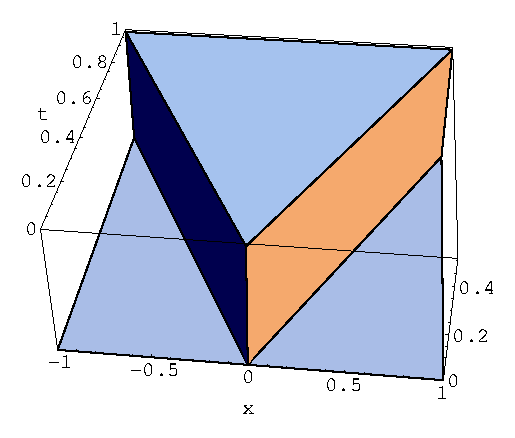
\includegraphics[width=0.4\textwidth]{pde/green/green_wave_mii}
    \end{center}
    \caption{Green function for the wave equation.}
    \label{green_wave_mii}
  \end{figure}

  Now we solve the wave equation with a source.
  \begin{gather*}
    u_{t t} - c^2 u_{x x} = q(x,t), \quad u(x,0) = u_t(x,0) = 0
    \\
    u = \int_0^\infty \int_{-\infty}^\infty G(x,t|\xi,t) q(\xi,\tau) \,\dd \xi \,\dd \tau
    \\
    u = \int_0^\infty \int_{-\infty}^\infty  \frac{1}{2c} H(c (t-\tau) - |x - \xi| ) q(\xi,\tau) \,\dd \xi \,\dd \tau
    \\
    \boxed{
      u = \frac{1}{2c} \int_0^t \int_{x - c (t-\tau)}^{x + c (t-\tau)} q(\xi,\tau) \,\dd \xi \,\dd \tau
      }
  \end{gather*}
\end{Solution}









%%By reducing the problem to a series of one dimensional Green function
\begin{Solution}
  \begin{enumerate}
    %%
    %%
  \item
    We expand the Green function in eigenfunctions in $x$.
    \[
    G(\mathbf{x}; \mathbf{x}i) = \sum_{n = 1}^\infty a_n(y) 
    \sin \left( \frac{(2n-1)\pi x}{2 L} \right)
    \]
    We substitute the expansion into the differential equation.
    \[
    \nabla^2 \sum_{n = 1}^\infty a_n(y) 
    \sqrt{ \frac{2}{L} } \sin \left( \frac{(2n-1)\pi x}{2 L} \right) 
    = \delta(x - \xi) \delta(y - \psi)
    \]
    \begin{multline*}
      \sum_{n = 1}^\infty \left( a_n''(y) 
        - \left( \frac{(2n-1)\pi}{2 L} \right)^2 a_n(y) \right)
      \sqrt{ \frac{2}{L} } \sin \left( \frac{(2n-1)\pi x}{2 L} \right) 
      \\
      = \delta(y - \psi) \sum_{n = 1}^\infty 
      \sqrt{ \frac{2}{L} } \sin \left( \frac{(2n-1)\pi \xi}{2 L} \right) 
      \sqrt{ \frac{2}{L} } \sin \left( \frac{(2n-1)\pi x}{2 L}
      \right)
    \end{multline*}
    \[
    a_n''(y) - \left( \frac{(2n-1)\pi}{2 L} \right)^2 a_n(y) 
    = \sqrt{ \frac{2}{L} } \sin \left( \frac{(2n-1)\pi \xi}{2 L}
    \right) \delta(y - \psi)
    \]
    From the boundary conditions at $y = 0$ and $y = H$, we obtain 
    boundary conditions for the $a_n(y)$.
    \[
    a_n'(0) = a_n'(H) = 0.
    \]
    The solutions that satisfy the left and right boundary conditions are
    \[
    a_{n1} = \cosh \left( \frac{(2n-1)\pi y}{2 L} \right), \quad
    a_{n2} = \cosh \left( \frac{(2n-1)\pi (H-y)}{2 L} \right).
    \]
    The Wronskian of these solutions is
    \[
    W = - \frac{(2n-1) \pi}{2L} \sinh \left( \frac{(2n-1)\pi}{2} \right).
    \]
    Thus the solution for $a_n(y)$ is
    \[
    a_n(y) = \sqrt{ \frac{2}{L} } \sin \left( \frac{(2n-1)\pi \xi}{2 L} \right)
    \frac{ \cosh \left( \frac{(2n-1)\pi y_<}{2 L} \right) 
      \cosh \left( \frac{(2n-1)\pi (H-y_>)}{2 L} \right) }
    { - \frac{(2n-1) \pi}{2L} \sinh \left( \frac{(2n-1)\pi}{2}
      \right) }
    \]
    \begin{multline*}
      a_n(y) = - \frac{ 2 \sqrt{2 L} }{ (2n-1) \pi } 
      \csch \left( \frac{(2n-1)\pi}{2} \right)
      \cosh \left( \frac{(2n-1)\pi y_<}{2 L} \right) 
      \\
      \cosh \left( \frac{(2n-1)\pi (H-y_>)}{2 L} \right)
      \sin \left( \frac{(2n-1)\pi \xi}{2 L} \right).
    \end{multline*}
    This determines the Green function.
    \begin{multline*}
      G(\mathbf{x}; \mathbf{x}i) = - \frac{ 2 \sqrt{2 L} }{ \pi } \sum_{n = 1}^\infty 
      \frac{ 1 }{2n-1} 
      \csch \left( \frac{(2n-1)\pi}{2} \right)
      \cosh \left( \frac{(2n-1)\pi y_<}{2 L} \right) 
      \\
      \cosh \left( \frac{(2n-1)\pi (H-y_>)}{2 L} \right)
      \sin \left( \frac{(2n-1)\pi \xi}{2 L} \right)
      \sin \left( \frac{(2n-1)\pi x}{2 L} \right)
    \end{multline*}
    %%
    %%
  \item
    We seek a solution of the form
    \[
    G(\mathbf{x}; \mathbf{x}i) = \sum_{\substack{m=1\\n=1}}^\infty
    a_{mn}(z) \frac{2}{\sqrt{L H} }
    \sin \left( \frac{ m \pi x }{ L } \right)
    \sin \left( \frac{ n \pi y }{ H } \right).
    \]
    We substitute this into the differential equation.
    \[
    \nabla^2 \sum_{\substack{m=1\\n=1}}^\infty
    a_{mn}(z) \frac{2}{\sqrt{L H} }
    \sin \left( \frac{ m \pi x }{ L } \right)
    \sin \left( \frac{ n \pi y }{ H } \right)
    = \delta(x - \xi) \delta(y - \psi) \delta(z - \zeta)
    \]
    \begin{multline*}
      \sum_{\substack{m=1\\n=1}}^\infty
      \left( a_{m n}''(z) 
        - \left( \left( \frac{ m \pi }{ L } \right)^2 
          + \left( \frac{ n \pi }{ H } \right)^2 \right)
        a_{mn}(z) \right) \frac{2}{\sqrt{L H} }
      \sin \left( \frac{ m \pi x }{ L } \right)
      \sin \left( \frac{ n \pi y }{ H } \right) 
      \\
      = \delta(z - \zeta) \sum_{\substack{m=1\\n=1}}^\infty
      \frac{2}{\sqrt{L H} }
      \sin \left( \frac{ m \pi \xi }{ L } \right)
      \sin \left( \frac{ n \pi \psi }{ H } \right)
      \frac{2}{\sqrt{L H} }
      \sin \left( \frac{ m \pi x }{ L } \right)
      \sin \left( \frac{ n \pi y }{ H } \right)
    \end{multline*}
    \[
    a_{m n}''(z) 
    - \pi \left( \left( \frac{ m }{ L } \right)^2 
      + \left( \frac{ n }{ H } \right)^2 \right) a_{mn}(z)
    = \frac{2}{\sqrt{L H} }
    \sin \left( \frac{ m \pi \xi }{ L } \right)
    \sin \left( \frac{ n \pi \psi }{ H } \right)
    \delta(z - \zeta)
    \]
    From the boundary conditions on $G$, we obtain boundary conditions 
    for the $a_{m n}$.
    \[
    a_{m n}(0) = a_{m n}(W) = 0
    \]
    The solutions that satisfy the left and right boundary conditions are
    \[
    a_{m n 1} = \sinh \left( \sqrt{ \left( \frac{ m }{ L } \right)^2 
        + \left( \frac{ n }{ H } \right)^2 } \, \pi z \right), \quad
    a_{m n 2} = \sinh \left( \sqrt{ \left( \frac{ m }{ L } \right)^2 
        + \left( \frac{ n }{ H } \right)^2 } \, \pi (W-z) \right).
    \]
    The Wronskian of these solutions is
    \[
    W = - \sqrt{ \left( \frac{ m }{ L } \right)^2 
      + \left( \frac{ n }{ H } \right)^2 } \, \pi 
    \sinh \left( \sqrt{ \left( \frac{ m }{ L } \right)^2 
        + \left( \frac{ n }{ H } \right)^2 } \, \pi W \right).
    \]
    Thus the solution for $a_{m n}(z)$ is
    \begin{multline*}
      a_{m n}(z) = \frac{2}{\sqrt{L H} }
      \sin \left( \frac{ m \pi \xi }{ L } \right)
      \sin \left( \frac{ n \pi \psi }{ H } \right) 
      \\
      \frac{ \sinh \left( \sqrt{ \left( \frac{ m }{ L } \right)^2 
            + \left( \frac{ n }{ H } \right)^2 } \, \pi z_< \right)
        \sinh \left( \sqrt{ \left( \frac{ m }{ L } \right)^2 
            + \left( \frac{ n }{ H } \right)^2 } \, \pi (W-z_>) \right) }
      { - \sqrt{ \left( \frac{ m }{ L } \right)^2 
          + \left( \frac{ n }{ H } \right)^2 } \, \pi 
        \sinh \left( \sqrt{ \left( \frac{ m }{ L } \right)^2 
            + \left( \frac{ n }{ H } \right)^2 } \, \pi W \right) }
    \end{multline*}
    \begin{multline*}
      a_{m n}(z) = - \frac{2}{ \pi \lambda_{m n} \sqrt{L H} }
      \csch \left( \lambda_{m n} \pi W \right)
      \sin \left( \frac{ m \pi \xi }{ L } \right)
      \sin \left( \frac{ n \pi \psi }{ H } \right) 
      \\
      \sinh \left( \lambda_{m n} \pi z_< \right)
      \sinh \left( \lambda_{m n} \pi (W-z_>) \right),
    \end{multline*}
    where
    \[
    \lambda_{m n} = \sqrt{ \left( \frac{ m }{ L } \right)^2 
      + \left( \frac{ n }{ H } \right)^2 }.
    \]
    This determines the Green function.
    \begin{multline*}
      G(\mathbf{x}; \mathbf{x}i) = - \frac{4}{ \pi L H }
      \sum_{\substack{m=1\\n=1}}^\infty
      \frac{1}{ \lambda_{m n} }
      \csch \left( \lambda_{m n} \pi W \right)
      \sin \left( \frac{ m \pi \xi }{ L } \right)
      \sin \left( \frac{ m \pi x }{ L } \right) 
      \\
      \sin \left( \frac{ n \pi \psi }{ H } \right)
      \sin \left( \frac{ n \pi y }{ H } \right)
      \sinh \left( \lambda_{m n} \pi z_< \right)
      \sinh \left( \lambda_{m n} \pi (W-z_>) \right)
    \end{multline*}
    %%
    %%
    %%
    %%
    %%
  \item
    First we write the problem in circular coordinates.
    \begin{gather*}
      \nabla^2 G = \delta(\mathbf{x} - \mathbf{x}i) \\
      G_{r r} + \frac{1}{r} G_r + \frac{1}{r^2} G_{\theta \theta}
      = \frac{1}{r} \delta(r - \rho) \delta(\theta - \vartheta), \\
      G(r,0; \rho, \vartheta) = G(r,\pi; \rho, \vartheta) = 
      G(0,\theta; \rho, \vartheta) = G(a,\theta; \rho, \vartheta) = 0
    \end{gather*}
    Because the Green function vanishes at $\theta = 0$ and
    $\theta = \pi$ we expand it in a series of the form
    \[
    G = \sum_{n = 1}^\infty g_n(r) \sin (n \theta).
    \]
    We substitute the series into the differential equation.
    \begin{gather*}
      \sum_{n = 1}^\infty \left( g_n''(r) + \frac{1}{r} g_n'(r) 
        - \frac{n^2}{r^2} g_n(r) \right) \sin (n \theta)
      = \frac{1}{r} \delta(r - \rho) 
      \sum_{n = 1}^\infty \frac{2}{\pi} \sin(n \vartheta) \sin(n \theta) \\
      g_n''(r) + \frac{1}{r} g_n'(r) - \frac{n^2}{r^2} g_n(r) 
      = \frac{2}{\pi r} \sin(n \vartheta) \delta(r - \rho) 
    \end{gather*}
    From the boundary conditions on $G$, we obtain boundary conditions 
    for the $g_n$.
    \[
    g_n(0) = g_n(a) = 0
    \]
    The solutions that satisfy the left and right boundary conditions are
    \[
    g_{n1} = r^n, \quad
    g_{n2} = \left( \frac{r}{a} \right)^n - \left( \frac{a}{r} \right)^n.
    \]
    The Wronskian of these solutions is
    \[
    W = \frac{2 n a^n}{r}.
    \]
    Thus the solution for $g_n(r)$ is
    \begin{gather*}
      g_n(r) = \frac{2}{\pi \rho} \sin(n \vartheta) 
      \frac{ r_<^n \left( \left( \frac{r_>}{a} \right)^n 
          - \left( \frac{a}{r_>} \right)^n \right) }
      { \frac{2 n a^n}{\rho} } \\
      g_n(r) = \frac{1}{n \pi} \sin(n \vartheta) 
      \left( \frac{r_<}{a} \right)^n \left( \left( \frac{r_>}{a} \right)^n 
        - \left( \frac{a}{r_>} \right)^n \right).
    \end{gather*}
    This determines the solution.
    \[
    G = \sum_{n = 1}^\infty \frac{1}{n \pi} 
    \left( \frac{r_<}{a} \right)^n \left( \left( \frac{r_>}{a} \right)^n 
      - \left( \frac{a}{r_>} \right)^n \right)
    \sin(n \vartheta) \sin (n \theta)
    \]
    %%
    %%
    %%
    %%
    %%
  \item
    First we write the problem in circular coordinates.
    \begin{gather*}
      G_{r r} + \frac{1}{r} G_r + \frac{1}{r^2} G_{\theta \theta}
      = \frac{1}{r} \delta(r - \rho) \delta(\theta - \vartheta), \\
      G(r,0; \rho, \vartheta) = G(r,\pi/2; \rho, \vartheta) = 
      G(0,\theta; \rho, \vartheta) = G_r(a,\theta; \rho, \vartheta) = 0
    \end{gather*}
    Because the Green function vanishes at $\theta = 0$ and
    $\theta = \pi/2$ we expand it in a series of the form
    \[
    G = \sum_{n = 1}^\infty g_n(r) \sin (2 n \theta).
    \]
    We substitute the series into the differential equation.
    \begin{gather*}
      \sum_{n = 1}^\infty \left( g_n''(r) + \frac{1}{r} g_n'(r) 
        - \frac{4 n^2}{r^2} g_n(r) \right) \sin (2 n \theta)
      = \frac{1}{r} \delta(r - \rho) 
      \sum_{n = 1}^\infty \frac{4}{\pi} \sin(2 n \vartheta) \sin(2 n \theta) \\
      g_n''(r) + \frac{1}{r} g_n'(r) - \frac{4 n^2}{r^2} g_n(r) 
      = \frac{4}{\pi r} \sin(2 n \vartheta) \delta(r - \rho) 
    \end{gather*}
    From the boundary conditions on $G$, we obtain boundary conditions 
    for the $g_n$.
    \[
    g_n(0) = g_n'(a) = 0
    \]
    The solutions that satisfy the left and right boundary conditions are
    \[
    g_{n1} = r^{2 n}, \quad
    g_{n2} = \left( \frac{r}{a} \right)^{2 n} 
    +  \left( \frac{a}{r} \right)^{2 n}.
    \]
    The Wronskian of these solutions is
    \[
    W = - \frac{4 n a^{2 n}}{r}.
    \]
    Thus the solution for $g_n(r)$ is
    \begin{gather*}
      g_n(r) = \frac{4}{\pi \rho} \sin(2 n \vartheta) 
      \frac{ r_<^{2 n} \left( \left( \frac{r_>}{a} \right)^{2 n} 
          +  \left( \frac{a}{r_>} \right)^{2 n} \right) }
      { - \frac{4 n a^{2 n}}{\rho} } \\
      g_n(r) = - \frac{ 1 }{\pi n} \sin(2 n \vartheta) 
      \left( \frac{r_<}{a} \right)^{2 n} 
      \left( \left( \frac{r_>}{a} \right)^{2 n} 
        +  \left( \frac{a}{r_>} \right)^{2 n} \right)
    \end{gather*}
    This determines the solution.
    \[
    G = - \sum_{n = 1}^\infty \frac{ 1 }{ \pi n } 
    \left( \frac{r_<}{a} \right)^{2 n}
    \left( \left( \frac{r_>}{a} \right)^{2 n} 
      +  \left( \frac{a}{r_>} \right)^{2 n} \right)
    \sin(2 n \vartheta) \sin (2 n \theta)
    \]
  \end{enumerate}
\end{Solution}










%% multi-dimensional eigenfunction.  \nabla^2  G = \delta(\mathbf{x}-\mathbf{x}_0)
\begin{Solution}
  \begin{enumerate}
    %%
    %%
    %%
    %%
  \item
    The set 
    \[
    \left\{ X_n \right\} = \left\{ 
      \sin \left( \frac{(2m-1) \pi x}{2 L} \right) \right\}_{m=1}^\infty
    \]
    are eigenfunctions of $\nabla^2$ and satisfy the boundary conditions
    $X_n(0) = X_n'(L) = 0$.  The set
    \[
    \left\{ Y_n \right\} = \left\{ 
      \cos \left( \frac{n \pi y}{H} \right) \right\}_{n=0}^\infty
    \]
    are eigenfunctions of $\nabla^2$ and satisfy the boundary conditions
    $Y_n'(0) = Y_n'(H) = 0$.  The set
    \[
    \left\{ \sin \left( \frac{(2m-1) \pi x}{2 L} \right) 
      \cos \left( \frac{n \pi y}{H} \right) 
    \right\}_{m=1,n=0}^\infty
    \]
    are eigenfunctions of $\nabla^2$ and satisfy the boundary conditions
    of this problem.  We expand the Green function in a series of these 
    eigenfunctions.
    \[
    G = \sum_{m = 1}^\infty g_{m0} \sqrt{ \frac{2}{L H} } \sin \left(
      \frac{ (2m-1) \pi x }{ 2 L } \right)
    + \sum_{\substack{m=1\\n=1}}^\infty g_{m n} 
    \frac{2}{\sqrt{L H}} \sin \left( \frac{ (2m-1) \pi x }{ 2 L } \right)
    \cos \left( \frac{ n \pi y }{ H } \right)
    \]
    We substitute the series into the Green function differential
    equation.
    \[
    \Delta G = \delta(x - \xi) \delta(y - \psi)
    \]
    \begin{multline*}
      - \sum_{m = 1}^\infty g_{m0} \left( \frac{ (2m-1) \pi }{ 2 L } \right)^2
      \sqrt{ \frac{2}{L H} } \sin \left(
        \frac{ (2m-1) \pi x }{ 2 L } \right) 
      \\
      - \sum_{\substack{m=1\\n=1}}^\infty g_{m n} 
      \left( \left( \frac{ (2m-1) \pi }{ 2 L } \right)^2
        + \left( \frac{ n \pi y }{ H } \right)^2 \right)
      \frac{2}{\sqrt{L H}} \sin \left( \frac{ (2m-1) \pi x }{ 2 L } \right)
      \cos \left( \frac{ n \pi y }{ H } \right) 
      \\
      = \sum_{m = 1}^\infty \sqrt{ \frac{2}{L H} } \sin \left(
        \frac{ (2m-1) \pi \xi }{ 2 L } \right)
      \sqrt{ \frac{2}{L H} } \sin \left(
        \frac{ (2m-1) \pi x }{ 2 L } \right) 
      \\
      + \sum_{\substack{m=1\\n=1}}^\infty 
      \frac{2}{\sqrt{L H}} \sin \left( \frac{ (2m-1) \pi \xi }{ 2 L } \right)
      \cos \left( \frac{ n \pi \psi }{ H } \right)
      \frac{2}{\sqrt{L H}} \sin \left( \frac{ (2m-1) \pi x }{ 2 L } \right)
      \cos \left( \frac{ n \pi y }{ H } \right)
    \end{multline*}
    We equate terms and solve for the coefficients $g_{m n}$.
    \begin{gather*}
      g_{m 0} = - \sqrt{ \frac{2}{L H} } 
      \left( \frac{ 2 L }{ (2m-1) \pi } \right)^2
      \sin \left( \frac{ (2m-1) \pi \xi }{ 2 L } \right) \\
      %%
      g_{m n} = - \frac{2}{\sqrt{L H}} 
      \frac{1}{ \pi^2 \left( \left( \frac{2m-1}{2L} \right)^2
          + \left( \frac{n}{H} \right)^2 \right) }
      \sin \left( \frac{ (2m-1) \pi \xi }{ 2 L } \right)
      \cos \left( \frac{ n \pi \psi }{ H } \right)
    \end{gather*}
    This determines the Green function.
    %%
    %%
    %%
    %%
  \item
    Note that 
    \[
    \left\{ \sqrt{ \frac{8}{L H W} }\,
      \sin \left( \frac{k \pi x}{L} \right),
      \sin \left( \frac{m \pi y}{H} \right),
      \sin \left( \frac{n \pi z}{W} \right) \ :\ 
      k,m,n \in \mathbb{Z}^+ \right\}
    \]
    is orthonormal and complete on 
    $(0 \ldots L) \times (0 \ldots H) \times (0 \ldots W)$.
    The functions are eigenfunctions of $\nabla^2$. 
    We expand the Green function in a series of these eigenfunctions.
    \[
    G = \sum_{k,m,n = 1}^\infty g_{k m n} \sqrt{ \frac{8}{L H W} }\,
    \sin \left( \frac{k \pi x}{L} \right)
    \sin \left( \frac{m \pi y}{H} \right)
    \sin \left( \frac{n \pi z}{W} \right)
    \]
    We substitute the series into the Green function differential
    equation.
    \[
    \Delta G = \delta(x - \xi) \delta(y - \psi) \delta(z - \zeta)
    \]
    \begin{multline*}
      - \sum_{k,m,n = 1}^\infty g_{k m n} 
      \left( \left( \frac{k \pi}{L} \right)^2 
        + \left( \frac{m \pi}{H} \right)^2
        +\left( \frac{n \pi}{W} \right)^2 \right)
      \sqrt{ \frac{8}{L H W} }\,
      \sin \left( \frac{k \pi x}{L} \right)
      \sin \left( \frac{m \pi y}{H} \right)
      \sin \left( \frac{n \pi z}{W} \right) 
      \\
      = \sum_{k,m,n = 1}^\infty 
      \sqrt{ \frac{8}{L H W} }\,
      \sin \left( \frac{k \pi \xi}{L} \right)
      \sin \left( \frac{m \pi \psi}{H} \right)
      \sin \left( \frac{n \pi \zeta}{W} \right) 
      \\
      \sqrt{ \frac{8}{L H W} }\,
      \sin \left( \frac{k \pi x}{L} \right)
      \sin \left( \frac{m \pi y}{H} \right)
      \sin \left( \frac{n \pi z}{W} \right)
    \end{multline*}
    We equate terms and solve for the coefficients $g_{k m n}$.
    \[
    g_{k m n} = - \frac{ \sqrt{ \frac{8}{L H W} }\,
      \sin \left( \frac{k \pi \xi}{L} \right)
      \sin \left( \frac{m \pi \psi}{H} \right)
      \sin \left( \frac{n \pi \zeta}{W} \right) }
    { \pi^2 \left( \left( \frac{k}{L} \right)^2 
        + \left( \frac{m}{H} \right)^2
        + \left( \frac{n}{W} \right)^2 \right) }
    \]
    This determines the Green function.
    %%
    %%
    %%
    %%
    %%
  \item
    The Green function problem is 
    \[
    \Delta G \equiv G_{r r} + \frac{1}{r} G_r 
    + \frac{1}{r^2} G_{\theta \theta} 
    = \frac{1}{r} \delta(r - \rho) \delta(\theta - \vartheta).
    \]
    We seek a set of functions $\{ \Theta_n(\theta) R_{n m}(r) \}$ which
    are orthogonal and complete on $(0 \ldots a) \times (0 \ldots \pi)$
    and which are eigenfunctions of the laplacian.  For the $\Theta_n$
    we choose eigenfunctions of $\frac{\partial^2}{\partial \theta^2}$.
    \begin{gather*}
      \Theta'' = - \nu^2 \Theta, \quad \Theta(0) = \Theta(\pi) = 0 \\
      %%
      \nu_n = n, \quad \Theta_n = \sin(n \theta), \quad n \in \mathbb{Z}^+ \\
    \end{gather*}
    Now we look for eigenfunctions of the laplacian.
    \begin{gather*}
      (R \Theta_n)_{r r} + \frac{1}{r} (R \Theta_n)_r 
      + \frac{1}{r^2} (R \Theta_n)_{\theta \theta} 
      = - \mu^2 R \Theta_n \\
      %%
      R'' \Theta_n + \frac{1}{r} R' \Theta_n 
      - \frac{n^2}{r^2} R \Theta_n = - \mu^2 R \Theta_n \\
      %%
      R'' + \frac{1}{r} R' + \left( \mu^2 - \frac{n^2}{r^2} \right) R = 0,
      \quad R(0) = R(a) = 0
    \end{gather*}
    The general solution for $R$ is
    \[
    R = c_1 J_n(\mu r) + c_2 Y_n(\mu r).
    \]
    the solution that satisfies the left boundary condition is
    $R = c J_n(\mu r)$.  We use the right boundary condition to 
    determine the eigenvalues.
    \[
    \mu_m = \frac{j_{n,m}}{a}, \quad
    R_{n m} = J_n \left( \frac{j_{n,m} r}{a} \right), \quad
    m,n \in \mathbb{Z}^+
    \]
    here $j_{n,m}$ is the $m^{\mathrm{th}}$ root of $J_n$.

    Note that 
    \[
    \left\{ \sin(n \theta) J_n \left( \frac{j_{n,m} r}{a} \right) \ :\ 
      m,n \in \mathbb{Z}^+ \right\}
    \]
    is orthogonal and complete on 
    $(r, \theta) \in (0 \ldots a) \times (0 \ldots \pi)$.
    We use the identities
    \[
    \int_0^\pi \sin^2 (n \theta) \,\dd \theta = \frac{\pi}{2}, \quad
    \int_0^1 r J_n^2(j_{n,m} r) \,\dd r = \frac{1}{2} J_{n+1}^2(j_{n,m})
    \]
    to make the functions orthonormal.
    \[
    \left\{ \frac{ 2 }{ \sqrt{\pi}\, a |J_{n+1}(j_{n,m})| }
      \sin(n \theta) J_n \left( \frac{j_{n,m} r}{a} \right) \ :\ 
      m,n \in \mathbb{Z}^+ \right\}
    \]
    We expand the Green function in a series of these eigenfunctions.
    \[
    G = \sum_{n,m = 1}^\infty g_{n m} \frac{ 2 }{ \sqrt{\pi}\, a |J_{n+1}(j_{n,m})| }
    J_n \left( \frac{j_{n,m} r}{a} \right) \sin(n \theta)
    \]
    We substitute the series into the Green function differential
    equation.
    \[
    G_{r r} + \frac{1}{r} G_r + \frac{1}{r^2} G_{\theta \theta} 
    = \frac{1}{r} \delta(r - \rho) \delta(\theta - \vartheta)
    \]
    \begin{multline*}
      - \sum_{n,m = 1}^\infty \left( \frac{j_{n,m}}{a} \right)^2
      g_{n m} \frac{ 2 }{ \sqrt{\pi}\, a |J_{n+1}(j_{n,m})| }
      J_n \left( \frac{j_{n,m} r}{a} \right) \sin(n \theta) 
      \\
      = \sum_{n,m = 1}^\infty \frac{ 2 }{ \sqrt{\pi}\, a |J_{n+1}(j_{n,m})| }
      J_n \left( \frac{j_{n,m} \rho}{a} \right) \sin(n \vartheta)
      \frac{ 2 }{ \sqrt{\pi}\, a |J_{n+1}(j_{n,m})| }
      J_n \left( \frac{j_{n,m} r}{a} \right) \sin(n \theta)
    \end{multline*}
    We equate terms and solve for the coefficients $g_{m n}$.
    \[
    g_{n m} = - \left( \frac{a}{j_{n,m}} \right)^2
    \frac{ 2 }{ \sqrt{\pi}\, a |J_{n+1}(j_{n,m})| }
    J_n \left( \frac{j_{n,m} \rho}{a} \right) \sin(n \vartheta)
    \]
    This determines the green function.
    %%
    %%
    %%
    %%
    %%
  \item
    The Green function problem is 
    \[
    \Delta G \equiv G_{r r} + \frac{1}{r} G_r 
    + \frac{1}{r^2} G_{\theta \theta} 
    = \frac{1}{r} \delta(r - \rho) \delta(\theta - \vartheta).
    \]
    We seek a set of functions $\{ \Theta_n(\theta) R_{n m}(r) \}$ which
    are orthogonal and complete on $(0 \ldots a) \times (0 \ldots \pi/2)$
    and which are eigenfunctions of the laplacian.  For the $\Theta_n$
    we choose eigenfunctions of $\frac{\partial^2}{\partial \theta^2}$.
    \begin{gather*}
      \Theta'' = - \nu^2 \Theta, \quad \Theta(0) = \Theta(\pi/2) = 0 \\
      %%
      \nu_n = 2 n, \quad \Theta_n = \sin(2 n \theta), \quad n \in \mathbb{Z}^+ \\
    \end{gather*}
    Now we look for eigenfunctions of the laplacian.
    \begin{gather*}
      (R \Theta_n)_{r r} + \frac{1}{r} (R \Theta_n)_r 
      + \frac{1}{r^2} (R \Theta_n)_{\theta \theta} 
      = - \mu^2 R \Theta_n \\
      %%
      R'' \Theta_n + \frac{1}{r} R' \Theta_n 
      - \frac{(2 n)^2}{r^2} R \Theta_n = - \mu^2 R \Theta_n \\
      %%
      R'' + \frac{1}{r} R' + \left( \mu^2 - \frac{(2 n)^2}{r^2} \right) R = 0,
      \quad R(0) = R(a) = 0
    \end{gather*}
    The general solution for $R$ is
    \[
    R = c_1 J_{2 n}(\mu r) + c_2 Y_{2 n}(\mu r).
    \]
    the solution that satisfies the left boundary condition is
    $R = c J_{2 n}(\mu r)$.  We use the right boundary condition to 
    determine the eigenvalues.
    \[
    \mu_m = \frac{{j'}_{2n,m}}{a}, \quad
    R_{n m} = J_{2 n} \left( \frac{{j'}_{2n,m} r}{a} \right), \quad
    m,n \in \mathbb{Z}^+
    \]
    here ${j'}_{n,m}$ is the $m^{\mathrm{th}}$ root of ${J'}_n$.

    Note that 
    \[
    \left\{ \sin(2 n \theta) {J'}_{2n} \left( \frac{{j'}_{2n,m} r}{a} \right) \ :\ 
      m,n \in \mathbb{Z}^+ \right\}
    \]
    is orthogonal and complete on 
    $(r, \theta) \in (0 \ldots a) \times (0 \ldots \pi/2)$.
    We use the identities
    \begin{gather*}
      \int_0^\pi \sin(m \theta) \sin(n \theta) \,\dd \theta 
      = \frac{\pi}{2} \delta_{m n}, \\
      \int_0^1 r J_\nu({j'}_{\nu,m} r) J_\nu({j'}_{\nu,n} r) \,\dd r 
      = \frac{{j'}_{\nu,n}^2 - \nu^2}{2 {j'}_{\nu,n}^2} 
      \left( J_\nu({j'}_{\nu,n}) \right)^2
      \delta_{m n}
    \end{gather*}
    to make the functions orthonormal.
    \[
    \left\{ \frac{ 2 {j'}_{2n,m} }
      { \sqrt{\pi}\, a \sqrt{{j'}_{2n,m}^2 - 4 n^2} |J_{2n}({j'}_{2n,m})| }
      \sin(2n \theta) J_{2n} \left( \frac{{j'}_{2n,m} r}{a} \right) \ :\ 
      m,n \in \mathbb{Z}^+ \right\}
    \]
    We expand the Green function in a series of these eigenfunctions.
    \[
    G = \sum_{n,m = 1}^\infty g_{n m} \frac{ 2 {j'}_{2n,m} }
    { \sqrt{\pi}\, a \sqrt{{j'}_{2n,m}^2 - 4 n^2} |J_{2n}({j'}_{2n,m})| }
    J_{2n} \left( \frac{{j'}_{2n,m} r}{a} \right) \sin(2n \theta) 
    \]
    We substitute the series into the Green function differential
    equation.
    \[
    G_{r r} + \frac{1}{r} G_r + \frac{1}{r^2} G_{\theta \theta} 
    = \frac{1}{r} \delta(r - \rho) \delta(\theta - \vartheta)
    \]
    \begin{multline*}
      - \sum_{n,m = 1}^\infty \left( \frac{{j'}_{2n,m}}{a} \right)^2
      g_{n m} \frac{ 2 {j'}_{2n,m} }
      { \sqrt{\pi}\, a \sqrt{{j'}_{2n,m}^2 - 4 n^2} |J_{2n}({j'}_{2n,m})| }
      J_{2n} \left( \frac{{j'}_{2n,m} r}{a} \right) \sin(2n \theta) 
      \\
      = \sum_{n,m = 1}^\infty \frac{ 2 {j'}_{2n,m} }
      { \sqrt{\pi}\, a \sqrt{{j'}_{2n,m}^2 - 4 n^2} |J_{2n}({j'}_{2n,m})| }
      J_{2n} \left( \frac{{j'}_{2n,m} \rho}{a} \right) \sin(2n
      \vartheta) 
      \\
      \frac{ 2 {j'}_{2n,m} }
      { \sqrt{\pi}\, a \sqrt{{j'}_{2n,m}^2 - 4 n^2} |J_{2n}({j'}_{2n,m})| }
      J_{2n} \left( \frac{{j'}_{2n,m} r}{a} \right) \sin(2n \theta)
    \end{multline*}
    We equate terms and solve for the coefficients $g_{m n}$.
    \[
    g_{n m} = - \left( \frac{a}{{j'}_{2n,m}} \right)^2
    \frac{ 2 {j'}_{2n,m} }
    { \sqrt{\pi}\, a \sqrt{{j'}_{2n,m}^2 - 4 n^2} |J_{2n}({j'}_{2n,m})| }
    J_{2n} \left( \frac{{j'}_{2n,m} \rho}{a} \right) \sin(2n \vartheta)
    \]
    This determines the green function.

  \end{enumerate}
\end{Solution}






%% Using the method of images solve \nabla^2 G = \delta (\mathbf{x} - \mathbf{x}_0)
\begin{Solution}
  We start with the equation
  \[
  \nabla^2 G = \delta(x - \xi) \delta(y - \psi).
  \]
  We do an odd reflection across the $y$ axis so that 
  $G(0,y; \xi,\psi) = 0$.
  \[
  \nabla^2 G = \delta(x - \xi) \delta(y - \psi)
  - \delta(x + \xi) \delta(y - \psi)
  \]
  Then we do an even reflection across the $x$ axis so that
  $G_y(x,0; \xi,\psi) = 0$.
  \[
  \nabla^2 G = \delta(x - \xi) \delta(y - \psi)
  - \delta(x + \xi) \delta(y - \psi)
  + \delta(x - \xi) \delta(y + \psi)
  - \delta(x + \xi) \delta(y + \psi)
  \]
  We solve this problem using the infinite space Green function.
  \begin{multline*}
    G = \frac{1}{4 \pi} \ln \left( (x-\xi)^2 + (y-\psi)^2 \right)
    - \frac{1}{4 \pi} \ln \left( (x+\xi)^2 + (y-\psi)^2 \right) 
    \\
    + \frac{1}{4 \pi} \ln \left( (x-\xi)^2 + (y+\psi)^2 \right)
    - \frac{1}{4 \pi} \ln \left( (x+\xi)^2 + (y+\psi)^2 \right) 
  \end{multline*}
  \[
  G = \frac{1}{4 \pi} \ln \left( 
    \frac{ \left( (x-\xi)^2 + (y-\psi)^2 \right)
      \left( (x-\xi)^2 + (y+\psi)^2 \right) }
    { \left( (x+\xi)^2 + (y-\psi)^2 \right) 
      \left( (x+\xi)^2 + (y+\psi)^2 \right) } \right)
  \]
  Now we solve the boundary value problem.
  \begin{gather*}
    u(\xi,\psi) = \int_S \left( u(x,y) \frac{\partial G}{\partial n} 
      - G \frac{\partial u(x,y)}{\partial n} \right) \,\dd S
    + \int_V G \Delta u \,\dd V \\
    u(\xi,\psi) = \int_\infty^0 u(0,y) (-G_x(0,y;\xi,\psi)) \,\dd y
    + \int_0^\infty -G(x,0;\xi,\psi) (-u_y(x,0)) \,\dd x \\
    u(\xi,\psi) = \int_0^\infty g(y) G_x(0,y;\xi,\psi) \,\dd y
    + \int_0^\infty G(x,0;\xi,\psi) h(x) \,\dd x \\
    u(\xi,\psi) = - \frac{\xi}{\pi} \int_0^\infty \left(
      \frac{1}{\xi^2 + (y-\psi)^2} + \frac{1}{\xi^2 + (y+\psi)^2}
    \right) g(y) \,\dd y
    + \frac{1}{2 \pi} \int_0^\infty \ln \left( 
      \frac{ (x-\xi)^2 + \psi^2 }{ (x+\xi)^2 + \psi^2 }
    \right) h(x) \,\dd x \\
    u(x,y) = - \frac{x}{\pi} \int_0^\infty \left(
      \frac{1}{x^2 + (y-\psi)^2} + \frac{1}{x^2 + (y+\psi)^2}
    \right) g(\psi) \,\dd \psi
    + \frac{1}{2 \pi} \int_0^\infty \ln \left( 
      \frac{ (x-\xi)^2 + y^2 }{ (x+\xi)^2 + y^2 }
    \right) h(\xi) \,\dd \xi 
  \end{gather*}
\end{Solution}







%% Consider the wave equation defined on the half-line $x>0$:
\begin{Solution}
  First we find the infinite space Green function.
  \[
  G_{t t} - c^2 G_{x x} = \delta(x - \xi) \delta(t - \tau), \quad
  G = G_t = 0\ \mathrm{for}\ t < \tau
  \]
  We solve this problem with the Fourier transform.
  \begin{gather*}
    \hat{G}_{t t} + c^2 \omega^2 \hat{G} 
    = \mathcal{F}[\delta(x-\xi)] \delta(t-\tau) \\
    \hat{G} = \mathcal{F}[\delta(x-\xi)] H(t-\tau) \frac{1}{c \omega}
    \sin( c \omega (t - \tau)) \\
    \hat{G} = H(t-\tau) \mathcal{F}[\delta(x-\xi)] 
    \mathcal{F} \left[ \frac{\pi}{c} H(c (t-\tau) - |x|) \right] \\
    G = H(t-\tau) \frac{\pi}{c} \frac{1}{2\pi} \int_{-\infty}^\infty
    \delta(y - \xi) H(c (t-\tau) - |x - y| ) \,\dd y \\
    G = \frac{1}{2c} H(t-\tau) H(c (t-\tau) - |x - \xi| ) \\
    G = \frac{1}{2c} H(c (t-\tau) - |x - \xi| )
  \end{gather*}

  \begin{enumerate}
    %%
    %%
    %%
    %%
  \item
    So that the Green function vanishes at $x = 0$ we do an odd reflection
    about that point.
    \begin{gather*}
      G_{t t} - c^2 G_{x x} = \delta(x - \xi) \delta(t - \tau)
      - \delta(x + \xi) \delta(t - \tau) \\
      G = \frac{1}{2c} H(c (t-\tau) - |x - \xi| )
      - \frac{1}{2c} H(c (t-\tau) - |x + \xi| )
    \end{gather*}
    %%
    %%
    %%
    %%
  \item
    Note that the Green function satisfies the symmetry relation
    \[
    G(x,t;\xi,\tau) = G(\xi,-\tau; x,-t).
    \]
    This implies that
    \[
    G_{x x} = G_{\xi \xi}, \quad G_{t t} = G_{\tau \tau}.
    \]
    We write the Green function problem and the inhomogeneous differential
    equation for $u$ in terms of $\xi$ and $\tau$.
    \begin{gather}
      \label{G_tautau-c^2G_xixi=delta(x-xi)delta(t-tau)}
      G_{\tau \tau} - c^2 G_{\xi \xi} = \delta(x-\xi) \delta(t-\tau) \\
      \label{u_tautau-c^2u_xixi=Q(xi,tau)}
      u_{\tau \tau} - c^2 u_{\xi \xi} = Q(\xi, \tau)
    \end{gather}
    We take the difference of $u$ times 
    Equation~\ref{G_tautau-c^2G_xixi=delta(x-xi)delta(t-tau)}
    and $G$ times Equation~\ref{u_tautau-c^2u_xixi=Q(xi,tau)}
    and integrate this over the domain $(0,\infty) \times (0,t^+)$.
    \begin{gather*}
      \int_0^{t^+} \int_0^\infty \left( u \delta(x-\xi) \delta(t-\tau) - G Q 
      \right) \,\dd \xi \,\dd \tau
      = \int_0^{t^+} \int_0^\infty \left( 
        u G_{\tau \tau} - u_{\tau \tau} G
        - c^2 \left( u G_{\xi \xi} - u_{\xi \xi} G \right) \right)
      \,\dd \xi \,\dd \tau \\
      %%
      u(x,t) = \int_0^{t^+} \int_0^\infty G Q \,\dd \xi \,\dd \tau
      + \int_0^{t^+} \int_0^\infty \left( 
        \frac{\partial}{\partial \tau} \left( u G_{\tau} - u_{\tau} G \right)
        - c^2 \frac{\partial}{\partial \xi} \left( u G_\xi - u_\xi G \right)
      \right) \,\dd \xi \,\dd \tau \\
      %%
      u(x,t) = \int_0^{t^+} \int_0^\infty G Q \,\dd \xi \,\dd \tau
      + \int_0^\infty \left[ u G_{\tau} - u_{\tau} G \right]_0^{t+} \,\dd \xi
      - c^2 \int_0^{t^+} \left[ u G_\xi - u_\xi G \right]_0^\infty \,\dd \tau \\
      %%
      u(x,t) = \int_0^{t^+} \int_0^\infty G Q \,\dd \xi \,\dd \tau
      - \int_0^\infty \left[ u G_{\tau} - u_{\tau} G \right]_{\tau = 0} \,\dd \xi
      + c^2 \int_0^{t^+} \left[ u G_\xi \right]_{\xi = 0} \,\dd \tau
    \end{gather*}
    We consider the case $Q(x,t) = f(x) = g(x) = 0$.
    \[
    u(x,t) = c^2 \int_0^{t^+} h(\tau) G_\xi(x,t; 0,\tau) \,\dd \tau
    \]
    We calculate $G_\xi$.
    \begin{gather*}
      G = \frac{1}{2c} \left( H(c (t-\tau) - |x - \xi| )
        - H(c (t-\tau) - |x + \xi| ) \right) \\
      G_\xi = \frac{1}{2c} \left( 
        \delta(c (t-\tau) - |x - \xi| ) (-1) \sign(x-\xi) (-1)
        - \delta(c (t-\tau) - |x + \xi| ) (-1) \sign(x+\xi) \right) \\
      G_\xi(x,t;0,\psi) = \frac{1}{c}    \delta(c (t-\tau) - |x| ) \sign(x) \\
      \intertext{We are interested in $x > 0$.}
      G_\xi(x,t;0,\psi) = \frac{1}{c}    \delta(c (t-\tau) - x ) 
    \end{gather*}
    Now we can calculate the solution $u$.
    \begin{gather*}
      u(x,t) = c^2 \int_0^{t^+} h(\tau) 
      \frac{1}{c} \delta(c (t-\tau) - x ) \,\dd \tau \\
      u(x,t) = \int_0^{t^+} h(\tau) 
      \delta \left((t-\tau) - \frac{x}{c} \right) \,\dd \tau \\
      u(x,t) = h \left( t - \frac{x}{c} \right)
    \end{gather*}
    %%
    %%
    %%
    %%
  \item
    The boundary condition influences the solution $u(x_1,t_1)$ only
    at the point $t = t_1 - x_1 / c$.  The contribution from the boundary
    condition $u(0,t) = h(t)$ is a wave moving to the right with 
    speed $c$.
  \end{enumerate}
\end{Solution}













\begin{Solution}
  \begin{gather*}
    g_{t t} - c^2 g_{x x} = 0, \quad
    g(x,0;\xi,\tau) = \delta(x - \xi), \quad 
    g_t(x,0;\xi,\tau) = 0 \\
    \hat{g}_{t t} + c^2 \omega^2 \hat{g}_{x x} = 0, \quad
    \hat{g}(x,0;\xi,\tau) = \mathcal{F}[\delta(x - \xi)], \quad 
    \hat{g}_t(x,0;\xi,\tau) = 0 \\
    \hat{g} = \mathcal{F}[\delta(x - \xi)] \cos(c \omega t) \\
    \hat{g} = \mathcal{F}[\delta(x - \xi)] 
    \mathcal{F}[\pi ( \delta(x + c t) + \delta(x - c t) ) ] \\
    g = \frac{1}{2\pi} \int_{-\infty}^\infty \delta(\psi - \xi) 
    \pi ( \delta(x - \psi + c t) + \delta(x - \psi - c t) ) \,\dd \psi \\
    \boxed{
      g(x,t; \xi) = \frac{1}{2} ( \delta(x - \xi + c t) 
      + \delta(x - \xi - c t) )
      }
  \end{gather*}
  \begin{gather*}
    \gamma_{t t} - c^2 \gamma_{x x} = 0, \quad
    \gamma(x,0;\xi,\tau) = 0, \quad 
    \gamma_t(x,0;\xi,\tau) = \delta(x - \xi) \\
    \hat{\gamma}_{t t} + c^2 \omega^2 \hat{\gamma}_{x x} = 0, \quad
    \hat{\gamma}(x,0;\xi,\tau) = 0, \quad 
    \hat{\gamma}_t(x,0;\xi,\tau) = \mathcal{F}[\delta(x - \xi)] \\
    \hat{\gamma} = \mathcal{F}[\delta(x - \xi)] 
    \frac{1}{c \omega} \sin(c \omega t) \\
    \hat{\gamma} = \mathcal{F}[\delta(x - \xi)] 
    \mathcal{F}\left[ \frac{\pi}{c} ( H(x + c t) + H(x - c t) ) \right] \\
    \gamma = \frac{1}{2\pi} \int_{-\infty}^\infty \delta(\psi - \xi) 
    \frac{\pi}{c} ( H(x - \psi + c t) + H(x - \psi - c t) ) \,\dd \psi \\
    \boxed{
      \gamma(x,t; \xi) = \frac{1}{2 c} ( H(x - \xi + c t) + H(x - \xi - c t) )
      }
  \end{gather*}
\end{Solution}





%% 1D wave equation on (-\infty..\infty) using Green functions.
\begin{Solution}
  \[
  u(x,t) = \int_0^\infty \int_{-\infty}^\infty G(x,t;\xi,\tau) f(\xi,\tau) \,\dd \xi \,\dd \tau 
  + \int_{-\infty}^\infty g(x,t;\xi) p(\xi) \,\dd \xi 
  + \int_{-\infty}^\infty \gamma(x,t;\xi) q(\xi) \,\dd \xi
  \]
  \begin{multline*}
    u(x, t) = \frac{1}{2 c} \int_0^\infty \int_{-\infty}^\infty H(t - \tau) (H(x - \xi + c(t - \tau))
    - H(x - \xi - c(t - \tau)) ) f(\xi, \tau) \,\dd \xi \,\dd \tau 
    \\
    + \frac{1}{2} \int_{-\infty}^\infty ( \delta(x - \xi + c t) 
    + \delta(x - \xi - c t) ) p(\xi) \,\dd \xi
    + \frac{1}{2 c} \int_{-\infty}^\infty ( H(x - \xi + c t) 
    + H(x - \xi - c t) ) q(\xi) \,\dd \xi 
  \end{multline*}
  \begin{multline*}
    u(x, t) = \frac{1}{2 c} \int_0^t \int_{-\infty}^\infty (H(x - \xi + c(t - \tau))
    - H(x - \xi - c(t - \tau)) ) f(\xi, \tau) \,\dd \xi \,\dd \tau 
    \\
    + \frac{1}{2} (p(x + c t) + p(x - c t))
    + \frac{1}{2 c} \int_{x - c t}^{x + c t} q(\xi) \,\dd \xi 
  \end{multline*}
  \[
  \boxed{
    u(x, t) = \frac{1}{2 c} \int_0^t \int_{x - c(t - \tau)}^{x + c(t - \tau)} 
    f(\xi, \tau) \,\dd \xi \,\dd \tau 
    + \frac{1}{2} (p(x + c t) + p(x - c t))
    + \frac{1}{2 c} \int_{x - c t}^{x + c t} q(\xi) \,\dd \xi 
    }
  \]

  This solution demonstrates the \textit{domain of dependence} of the
  solution.  The first term is an integral over the triangle domain
  $\{ (\xi,\tau) : 0 < \tau < t, x - c \tau < \xi < x + c \tau \}$.
  The second term involves only the points $(x \pm c t, 0)$.
  The third term is an integral on the line segment
  $\{ (\xi,0) : x - c t < \xi < x + c t \}$.
  In totallity, this is just the triangle domain.
  This is shown graphically in Figure~\ref{domain_of_dependence}.
  \begin{figure}[h!]
    \begin{center}
      \includegraphics[width=0.5\textwidth]{pde/green/domain_of_dependence}
    \end{center}
    \caption{Domain of dependence for the wave equation.}
    \label{domain_of_dependence}
  \end{figure}
\end{Solution}




%% Green function in a rectangle.
\begin{Solution}
  \textbf{Single Sum Representation.}
  First we find the eigenfunctions of the homogeneous problem
  $\Delta u - k^2 u = 0$.  We substitute the separation of variables,
  $u(x,y) = X(x) Y(y)$ into the partial differential equation.
  \begin{gather*}
    X'' Y + X Y'' - k^2 X Y = 0 \\
    \frac{X''}{X} = k^2 - \frac{Y''}{Y} = - \lambda^2
  \end{gather*}
  We have the regular Sturm-Liouville eigenvalue problem,
  \[
  X'' = - \lambda^2 X, \quad X(0) = X(a) = 0,
  \]
  which has the solutions,
  \[
  \lambda_n = \frac{n \pi}{a}, \quad
  X_n = \sin \left( \frac{n \pi x}{a} \right), \quad
  n \in \mathbb{N}.
  \]
  We expand the solution $u$ in a series of these eigenfunctions.
  \[
  G(x,y;\xi,\psi) = \sum_{n = 1}^\infty c_n(y) \sin \left( \frac{n \pi x}{a} \right)
  \]
  We substitute this series into the partial differential equation to 
  find equations for the $c_n(y)$.
  \[
  \sum_{n = 1}^\infty \left( - \left( \frac{n \pi}{a} \right)^2 c_n(y) + c_n''(y)
    - k^2 c_n(y) \right) \sin \left( \frac{n \pi x}{a} \right)
  = \delta(x - \xi) \delta(y - \psi)
  \]
  The series expansion of the right side is,
  \begin{gather*}
    \delta(x-\xi) \delta(y-\psi) = \sum_{n = 1}^\infty d_n(y) \sin \left(
      \frac{n \pi x}{a} \right) \\
    d_n(y) = \frac{2}{a} \int_0^a \delta(x-\xi) \delta(y-\psi)
    \sin \left( \frac{n \pi x}{a} \right) \,\dd x \\
    d_n(y) = \frac{2}{a} \sin \left( \frac{n \pi \xi}{a} \right) \delta(y-\psi).
  \end{gather*}
  The the equations for the $c_n(y)$ are
  \[
  c_n''(y) - \left( k^2 + \left( \frac{n \pi}{a} \right)^2 \right) c_n(y)
  = \frac{2}{a} \sin \left( \frac{n \pi \xi}{a} \right) \delta(y-\psi),
  \quad c_n(0) = c_n(b) = 0.
  \]
  The homogeneous solutions are $\{ \cosh(\sigma_n y), \sinh(\sigma_n y) \}$,
  where $\sigma_n = \sqrt{k^2 (n \pi/a)^2}$.  The solutions that satisfy 
  the boundary conditions at $y = 0$ and $y = b$ are, $\sinh(\sigma_n y)$
  and $\sinh(\sigma_n(y-b))$, respectively.  The Wronskian of these solutions
  is,
  \begin{align*}
    W(y)    &= \begin{vmatrix} \sinh(\sigma_n y) & \sinh(\sigma_n (y-b)) \\
      \sigma_n \cosh(\sigma_n y) & \sigma_n \cosh(\sigma_n(y-b))
    \end{vmatrix} \\
    &= \sigma_n \left( \sinh(\sigma_n y) \cosh( \sigma_n (y-b) )
      - \sinh( \sigma_n (y-b)) \cosh( \sigma_n y ) \right) \\
    &= \sigma_n \sinh( \sigma_n b ).
  \end{align*}
  The solution for $c_n(y)$ is
  \[
  c_n(y) = \frac{2}{a} \sin \left( \frac{n \pi \xi}{a} \right) 
  \frac{ \sinh(\sigma_n y_<) \sinh(\sigma_n (y_>-b)) }
  { \sigma_n \sinh( \sigma_n b ) }.
  \]
  The Green function for the partial differential equation is
  \[
  \boxed{
    G(x,y;\xi,\psi) = \frac{2}{a} \sum_{n = 1}^\infty 
    \frac{ \sinh(\sigma_n y_<) \sinh(\sigma_n(y_>-b)) }
    { \sigma_n \sinh(\sigma_n b) }
    \sin \left( \frac{n \pi x}{a} \right)
    \sin \left( \frac{n \pi \xi}{a} \right).
    }
  \]
\end{Solution}



%% Green function in quarter plane with mixed boundary conditions.
\begin{Solution}
  We take the Fourier cosine transform in $x$ of the partial differential 
  equation and the boundary condition along $y = 0$.
  \begin{gather*}
    G_{x x} + G_{y y} - k^2 G = \delta(x-\xi) \delta(y - \psi) \\
    - \alpha^2 \hat{G}(\alpha,y) - \frac{1}{\pi} \hat{G}_x(0,y)
    + \hat{G}_{y y}(\alpha,y) - k^2 \hat{G}(\alpha,y)
    = \frac{1}{\pi} \cos(\alpha \xi) \delta(y-\psi) \\
    \hat{G}_{y y}(\alpha,y) - (k^2 + \alpha^2) \hat{G}(\alpha,y) = 
    = \frac{1}{\pi} \cos(\alpha \xi) \delta(y-\psi), \quad
    \hat{G}(\alpha,0) = 0 \\
  \end{gather*}
  Then we take the Fourier sine transform in $y$.
  \begin{gather*}
    -\beta^2 \hat{\hat{G}}(\alpha,\beta) 
    + \frac{\beta}{\pi} \hat{\hat{G}}(\alpha,0) 
    - (k^2 + \alpha^2) \hat{\hat{G}}(\alpha,\beta) 
    = \frac{1}{\pi^2} \cos(\alpha\xi) \sin(\beta\psi) \\
    \hat{\hat{G}} = - \frac{ \cos(\alpha\xi) \sin(\beta\psi) }
    { \pi^2 (k^2 + \alpha^2 + \beta^2) }
  \end{gather*}
  We take two inverse transforms to find the solution.  For one integral 
  representation of the Green function we take the inverse sine transform
  followed by the inverse cosine transform.
  \begin{gather*}
    \hat{\hat{G}} = - \cos(\alpha\xi) \frac{\sin(\beta\psi)}{\pi}
    \frac{1}{\pi(k^2 + \alpha^2 + \beta^2)} 
    \\
    \hat{\hat{G}} = - \cos(\alpha\xi) \mathcal{F}_s [\delta(y-\psi)]
    \mathcal{F}_c \left[ \frac{1}{ \sqrt{k^2+\alpha^2} }
      \e^{ - \sqrt{ k^2 + \alpha^2 } y } \right] 
  \end{gather*}
  \begin{multline*}
    \hat{G}(\alpha,y) = - \cos(\alpha \xi) \frac{1}{2\pi} \int_0^\infty
    \delta(z-\psi) \frac{1}{\sqrt{k^2+\alpha^2}} \left(
      \exp\left( - \sqrt{k^2 + \alpha^2} |y-z| \right) \right.
    \\
    - \left. \exp\left( - \sqrt{k^2 + \alpha^2} (y+z) \right) \right) \,\dd z 
  \end{multline*}
  \begin{gather*}
    \hat{G}(\alpha,y) = - \frac{ \cos(\alpha \xi) }{ 2 \pi \sqrt{k^2 + \alpha^2} }
    \left( \exp\left( - \sqrt{k^2 + \alpha^2} |y-\psi| \right)
      - \exp\left( - \sqrt{k^2 + \alpha^2} (y+\psi) \right) \right) 
    \\
    \boxed{
      G(x,y;\xi,\psi) = - \frac{1}{\pi} \int_0^\infty 
      \frac{ \cos(\alpha \xi) }{ \sqrt{k^2 + \alpha^2} }
      \left( \exp\left( - \sqrt{k^2 + \alpha^2} |y-\psi| \right)
        - \exp\left( - \sqrt{k^2 + \alpha^2} (y+\psi) \right) \right) \,\dd \alpha
      }
  \end{gather*}
  For another integral representation of the Green function, we take the 
  inverse cosine transform followed by the inverse sine transform.
  \begin{gather*}
    \hat{\hat{G}}(\alpha,\beta) = - \sin(\beta\psi) \frac{\cos(\alpha\xi)}{\pi}
    \frac{1}{ \pi (k^2 + \alpha^2 + \beta^2) } \\
    \hat{\hat{G}}(\alpha,\beta) = - \sin(\beta\psi) 
    \mathcal{F}_c[ \delta(x-\xi) ]
    \mathcal{F}_c \left[ \frac{1}{\sqrt{k^2 + \beta^2}}
      \e^{-\sqrt{ k^2 + \beta^2 } x} \right] \\
    \hat{G}(x,\beta) = - \sin(\beta\psi) \frac{1}{2\pi} \int_0^\infty \delta(z - \xi)
    \frac{1}{\sqrt{ k^2 + \beta^2 } } \left(
      \e^{- \sqrt{k^2 + \beta^2} |x - z|} 
      + \e^{- \sqrt{k^2 + \beta^2} (x + z)} \right) \,\dd z \\
    \hat{G}(x,\beta) = - \sin(\beta\psi) \frac{1}{2\pi} 
    \frac{1}{\sqrt{ k^2 + \beta^2 } } \left(
      \e^{- \sqrt{k^2 + \beta^2} |x - \xi|} 
      + \e^{- \sqrt{k^2 + \beta^2} (x + \xi)} \right) \\
    \boxed{
      G(x,y;\xi,\psi) = - \frac{1}{\pi} \int_0^\infty
      \frac{\sin(\beta y) \sin(\beta \psi)}{\sqrt{ k^2 + \beta^2 } } \left(
        \e^{- \sqrt{k^2 + \beta^2} |x - \xi|} 
        + \e^{- \sqrt{k^2 + \beta^2} (x + \xi)} \right)\,\dd \beta
      }
  \end{gather*}
\end{Solution}






%% Green function on infinite sector.
\begin{Solution}
  The problem is:
  \begin{align*}
    &G_{r r} + \frac{1}{r} G_r + \frac{1}{r^2} G_{\theta\theta} = 
    \frac{ \delta(r-\rho) \delta(\theta-\vartheta) }{ r }, 
    \quad 0 < r < \infty, \quad 0 < \theta < \alpha, \\
    &G(r,0,\rho,\vartheta) = G(r,\alpha,\rho,\vartheta) = 0, \\
    &G(0,\theta,\rho,\vartheta) = 0 \\
    &G(r,\theta,\rho,\vartheta) \to 0\ \mathrm{as}\ r \to \infty.
  \end{align*}
  Let $w = r \e^{i \theta}$ and $z = x + i y$.  We use the conformal mapping,
  $z = w^{\pi/\alpha}$ to map the sector to the upper half $z$ plane.  The
  problem is $(x,y)$ space is
  \begin{align*}
    &G_{x x} + G_{y y} = \delta(x - \xi) \delta(y - \psi), 
    \quad -\infty < x < \infty, \quad 0 < y < \infty, \\
    &G(x,0,\xi,\psi) = 0, \\
    &G(x,y,\xi,\psi) \to 0\ \mathrm{as}\ x,y \to \infty.
  \end{align*}
  We will solve this problem with the method of images.  Note that the solution
  of,
  \begin{gather*}
    G_{x x} + G_{y y} = \delta(x-\xi) \delta(y-\psi) 
    - \delta(x-\xi) \delta(y+\psi), \quad - \infty < x < \infty,
    \quad - \infty < y < \infty, \\
    G(x,y,\xi,\psi) \to 0\ \mathrm{as}\ x,y \to \infty,
  \end{gather*}
  satisfies the condition, $G(x,0,\xi,\psi) = 0$.  Since the infinite space
  Green function for the Laplacian in two dimensions is
  \[
  \frac{1}{4\pi} \ln \left( (x-\xi)^2 + (y-\psi)^2 \right),
  \]
  the solution of this problem is,
  \begin{align*}
    G(x,y,\xi,\psi) &= 
    \frac{1}{4\pi} \ln \left( (x-\xi)^2 + (y-\psi)^2 \right)
    - \frac{1}{4\pi} \ln \left( (x-\xi)^2 + (y+\psi)^2 \right) \\
    &= \frac{1}{4\pi} \ln \left( \frac{ (x-\xi)^2 + (y-\psi)^2 }
      { (x-\xi)^2 + (y+\psi)^2 } \right).
  \end{align*}
  Now we solve for $x$ and $y$ in the conformal mapping.
  \begin{gather*}
    z = w^{\pi/\alpha} = (r \e^{i \theta})^{\pi/\alpha} \\
    x + i y = r^{\pi/\alpha} (\cos(\theta \pi/\alpha) + i\sin(\theta \pi/\alpha))\\
    x = r^{\pi/\alpha} \cos(\theta \pi / \alpha), \qquad
    y = r^{\pi/\alpha} \sin(\theta \pi / \alpha)
  \end{gather*}
  We substitute these expressions into $G(x,y,\xi,\psi)$ to obtain
  $G(r,\theta,\rho,\vartheta)$.
  \begin{align*}
    G(r,\theta,\rho,\vartheta)
    &= \frac{1}{4\pi} \ln \left(
      \frac{ ( r^{\pi/\alpha} \cos(\theta \pi/\alpha)
        - \rho^{\pi/\alpha} \cos(\vartheta \pi / \alpha) )^2
        + ( r^{\pi/\alpha} \sin(\theta \pi/\alpha)
        - \rho^{\pi/\alpha} \sin(\vartheta \pi / \alpha) )^2 }
      { ( r^{\pi/\alpha} \cos(\theta \pi/\alpha)
        - \rho^{\pi/\alpha} \cos(\vartheta \pi / \alpha) )^2
        + ( r^{\pi/\alpha} \sin(\theta \pi/\alpha)
        + \rho^{\pi/\alpha} \sin(\vartheta \pi / \alpha) )^2 } \right)\\
    &= \frac{1}{4\pi} \ln \left(
      \frac{ r^{2 \pi / \alpha} + \rho^{2 \pi / \alpha}
        - 2 r^{\pi/\alpha} \rho^{\pi/\alpha} 
        \cos( \pi(\theta-\vartheta) / \alpha ) }
      { r^{2 \pi / \alpha} + \rho^{2 \pi / \alpha}
        - 2 r^{\pi/\alpha} \rho^{\pi/\alpha} 
        \cos( \pi(\theta+\vartheta) / \alpha ) } \right) \\
    &= \frac{1}{4\pi} \ln \left(
      \frac{ (r/\rho)^{\pi/\alpha} / 2 + (\rho/r)^{\pi/\alpha} / 2
        - \cos( \pi(\theta-\vartheta) / \alpha ) }
      { (r/\rho)^{\pi/\alpha} / 2 + (\rho/r)^{\pi/\alpha} / 2
        - \cos( \pi(\theta+\vartheta) / \alpha ) } \right) \\
    &= \frac{1}{4\pi} \ln \left(
      \frac{ \e^{\pi \ln(r/\rho) / \alpha} / 2 
        + \e^{\pi \ln(\rho/r)/\alpha} / 2
        - \cos( \pi(\theta-\vartheta) / \alpha ) }
      { \e^{\pi \ln(r/\rho) / \alpha} / 2 
        + \e^{\pi \ln(\rho/r)/\alpha} / 2
        - \cos( \pi(\theta+\vartheta) / \alpha ) } \right) 
  \end{align*}
  \[
  \boxed{
    G(r,\theta,\rho,\vartheta) = \frac{1}{4\pi} \ln \left(
      \frac{ \cosh \left( \frac{\pi/\alpha} \ln \frac{r}{\rho} \right)
        - \cos( \pi(\theta-\vartheta) / \alpha ) }
      { \cosh \left( \frac{\pi/\alpha} \ln \frac{r}{\rho} \right)
        - \cos( \pi(\theta+\vartheta) / \alpha ) } \right)
    }
  \]
  Now recall that the solution of
  \[
  \Delta u = f(\mathbf{x}),
  \]
  subject to the boundary condition,
  \[
  u(\mathbf{x}) = g(\mathbf{x}),
  \]
  is
  \[
  u(\mathbf{x}) = \int \int f(\mathbf{x}i) G(\mathbf{x}; \mathbf{x}i) \,\dd A_\xi
  + \oint g(\mathbf{x}i) \nabla_\xi G(\mathbf{x}; \mathbf{x}i) \cdot \hat{\mathbf{n}} 
  \,\dd s_\xi.
  \]
  The normal directions along the lower and upper edges of the sector are
  $- \hat{\theta}$ and $\hat{\theta}$, respectively.  The gradient in
  polar coordinates is
  \[
  \nabla_\xi = \hat{\rho} \frac{\partial}{\partial \rho} + \frac{\hat{\vartheta}}{\rho}
  \frac{\partial }{\partial \vartheta}.
  \]
  We only need to compute the $\hat{\vartheta}$ component of the gradient of
  $G$.  This is
  \[
  \frac{1}{\rho} \frac{\partial}{\partial \rho} G = 
  \frac{ \sin(\pi(\theta-\vartheta)/\alpha) }
  { 4 \alpha \rho \left( \cosh \left( \frac{\pi}{\alpha} 
        \ln \frac{r}{\rho} \right) -\cos(\pi(\theta-\vartheta)/\alpha)\right)}
  + \frac{ \sin(\pi(\theta-\vartheta)/\alpha) }
  { 4 \alpha \rho \left( \cosh \left( \frac{\pi}{\alpha} 
        \ln \frac{r}{\rho} \right) -\cos(\pi(\theta+\vartheta)/\alpha)\right)}
  \]
  Along $\vartheta = 0$, this is
  \[
  \frac{1}{\rho} G_\vartheta(r,\theta,\rho,0) = 
  \frac{ \sin(\pi \theta/\alpha) }
  { 2 \alpha \rho \left( \cosh \left( \frac{\pi}{\alpha} 
        \ln \frac{r}{\rho} \right) -\cos(\pi \theta /\alpha)\right)}.
  \]
  Along $\vartheta = \alpha$, this is
  \[
  \frac{1}{\rho} G_\vartheta(r,\theta,\rho,\alpha) = 
  - \frac{ \sin(\pi \theta/\alpha) }
  { 2 \alpha \rho \left( \cosh \left( \frac{\pi}{\alpha} 
        \ln \frac{r}{\rho} \right) +\cos(\pi \theta /\alpha)\right)}.
  \]
  The solution of our problem is
  \begin{gather*}
    u(r,\theta) = \int_\infty^c
    - \frac{ \sin(\pi \theta/\alpha) }
    { 2 \alpha \rho \left( \cosh \left( \frac{\pi}{\alpha} 
          \ln \frac{r}{\rho} \right) +\cos(\pi \theta /\alpha)\right)} \,\dd \rho
    + \int_c^\infty 
    - \frac{ \sin(\pi \theta/\alpha) }
    { 2 \alpha \rho \left( \cosh \left( \frac{\pi}{\alpha} 
          \ln \frac{r}{\rho} \right) -\cos(\pi \theta /\alpha)\right)} \,\dd \rho\\
    u(r,\theta) = 
    \int_c^\infty 
    \frac{ - \sin(\pi \theta/\alpha) }
    { 2 \alpha \rho \left( \cosh \left( \frac{\pi}{\alpha} 
          \ln \frac{r}{\rho} \right) -\cos(\pi \theta /\alpha)\right)} 
    + \frac{ \sin(\pi \theta/\alpha) }
    { 2 \alpha \rho \left( \cosh \left( \frac{\pi}{\alpha} 
          \ln \frac{r}{\rho} \right) +\cos(\pi \theta /\alpha)\right)} \,\dd \rho\\
    u(r,\theta) = - \frac{1}{\alpha} \sin\left( \frac{\pi \theta}{\alpha} \right)
    \cos\left( \frac{\pi\theta}{\alpha} \right)
    \int_c^\infty 
    \frac{ 1 }{ \rho \left( \cosh^2 \left( \frac{\pi}{\alpha} 
          \ln \frac{r}{\rho} \right) -\cos^2 \left( \frac{\pi \theta}{\alpha}
        \right) \right) } \,\dd \rho \\
    u(r,\theta) = - \frac{1}{\alpha} \sin\left( \frac{\pi \theta}{\alpha} \right)
    \cos\left( \frac{\pi\theta}{\alpha} \right)
    \int_{\ln(c/r)}^\infty 
    \frac{ 1 }{ \cosh^2 \left( \frac{\pi x}{\alpha} \right)
      - \cos^2 \left( \frac{ \pi \theta }{\alpha} \right) } \,\dd x \\
    \boxed{
      u(r,\theta) = - \frac{2}{\alpha} \sin\left( \frac{\pi \theta}{\alpha} \right)
      \cos\left( \frac{\pi\theta}{\alpha} \right)
      \int_{\ln(c/r)}^\infty 
      \frac{ 1 }{ \cosh \left( \frac{2 \pi x}{\alpha} \right)
        - \cos \left( \frac{ 2 \pi \theta }{\alpha} \right) } \,\dd x
      }
  \end{gather*}
\end{Solution}









%% Heat equation, method of images
\begin{Solution}
  First consider the Green function for
  \[
  u_t - \kappa u_{x x} = 0, \quad u(x,0) = f(x).
  \]
  The differential equation and initial condition is
  \[
  G_t = \kappa G_{x x}, \quad G(x,0;\xi) = \delta(x - \xi).
  \]
  The Green function is a solution of the homogeneous heat equation for the 
  initial condition of a unit amount of heat concentrated at the point $x=\xi$.
  You can verify that the Green function is a solution of the heat equation 
  for $t>0$ and that it has the property:
  \[
  \int_{-\infty}^\infty G(x,t;\xi) \,\dd x = 1, \quad \mathrm{for}\ t > 0.
  \]
  This property demonstrates that the total amount of heat is the constant 1.
  At time $t=0$ the heat is concentrated at the point $x = \xi$.  As time 
  increases, the heat diffuses out from this point.

  The solution for $u(x,t)$ is the linear combination of the Green functions 
  that satisfies the initial condition $u(x,0) = f(x)$.  This linear combination
  is
  \[
  u(x,t) = \int_{-\infty}^\infty G(x,t;\xi) f(\xi) \,\dd \xi.
  \]
  $G(x,t;1)$ and $G(x,t;-1)$ are plotted in Figure~\ref{heatmii1am1} for the 
  domain $t \in [1/100..1/4]$, $x \in [-2..2]$ and $\kappa = 1$.

  \begin{figure}[h!]
    \begin{center}
      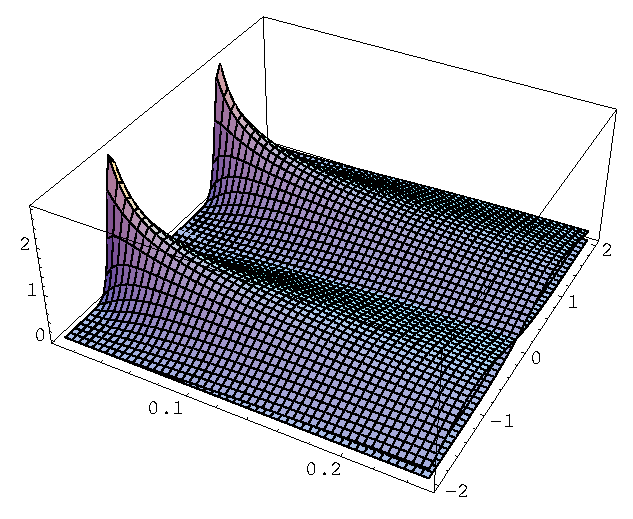
\includegraphics[width=0.5\textwidth]{pde/green/heatmii1am1}
    \end{center}
    \caption{The Green functions.}
    \label{heatmii1am1}
  \end{figure}

  Now we consider the problem
  \[
  u_t = \kappa u_{x x}, \quad u(x,0) = f(x)\ \mathrm{for}\ x > 0, \quad u(0,t) = 0.
  \]
  Note that the solution of 
  \begin{gather*}
    G_t = \kappa G_{x x}, \quad x > 0, \quad t > 0, \\
    G(x,0;\xi) = \delta(x-\xi) - \delta(x+\xi),
  \end{gather*}
  satisfies the boundary condition $G(0,t;\xi) = 0$.
  We write the solution as the difference of infinite space Green functions.
  \begin{align*}
    G(x,t;\xi) &= \frac{1}{\sqrt{4 \pi \kappa t}} \e^{-(x-\xi)^2  / (4 \kappa t)}
    - \frac{1}{\sqrt{4 \pi \kappa t}} \e^{-(x+\xi)^2 / (4 \kappa t)} \\
    &= \frac{1}{\sqrt{4 \pi \kappa t}} \left( 
      \e^{-(x-\xi)^2  / (4 \kappa t)}
      - \e^{-(x+\xi)^2 / (4 \kappa t)} \right) 
  \end{align*}
  \[
  \boxed{
    G(x,t;\xi) = \frac{1}{\sqrt{4 \pi \kappa t}} 
    \e^{-(x^2 + \xi^2) / (4 \kappa t)} 
    \sinh \left( \frac{x \xi}{2 \kappa t} \right)
    }
  \]

  Next we consider the problem
  \[
  u_t = \kappa u_{x x}, \quad u(x,0) = f(x)\ \mathrm{for}\ x > 0, 
  \quad u_x(0,t) = 0.
  \]
  Note that the solution of 
  \begin{gather*}
    G_t = \kappa G_{x x}, \quad x > 0, \quad t > 0, \\
    G(x,0;\xi) = \delta(x-\xi) + \delta(x+\xi),
  \end{gather*}
  satisfies the boundary condition $G_x(0,t;\xi) = 0$.
  We write the solution as the sum of infinite space Green functions.
  \begin{gather*}
    G(x,t;\xi) = \frac{1}{\sqrt{4 \pi \kappa t}} \e^{-(x-\xi)^2  / (4 \kappa t)}
    + \frac{1}{\sqrt{4 \pi \kappa t}} \e^{-(x+\xi)^2 / (4 \kappa t)} \\
    \boxed{
      G(x,t;\xi) = \frac{1}{\sqrt{4 \pi \kappa t}} 
      \e^{-(x^2 + \xi^2) / (4 \kappa t)} 
      \cosh \left( \frac{x \xi}{2 \kappa t} \right)
      }
  \end{gather*}

  The Green functions for the two boundary conditions are shown in 
  Figure~\ref{heatzi}.

  \begin{figure}[h!]
    \begin{center}
      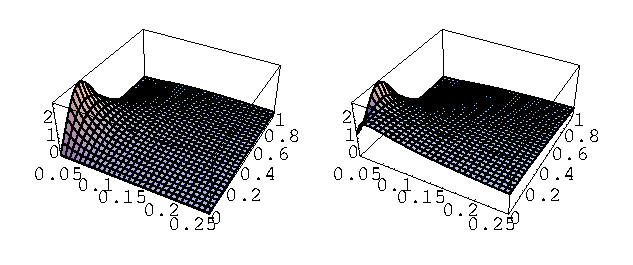
\includegraphics[width=\textwidth]{pde/green/heatzi}
    \end{center}
    \caption{Green functions for the two boundary conditions.}
    \label{heatzi}
  \end{figure}
\end{Solution}












%% Green function for 1D wave equation on 0..L.
\begin{Solution}
  $\phantom{a}$

  \textbf{a)}
  The Green function problem is
  \begin{gather*}
    G_{t t} - c^2 G_{x x} = \delta(t - \tau) \delta(x - \xi), \quad 0 < x < L,
    \quad t > 0, \\
    G(0, t; \xi, \tau) = G_x(L, t; \xi, \tau) = 0, \\
    G(x, t; \xi, \tau) = 0\ \mathrm{for}\ t < \tau.
  \end{gather*}
  The condition that $G$ is zero for $t < \tau$ makes this a \textit{causal}
  Green function.  We solve this problem by expanding $G$ in a series of 
  eigenfunctions of the $x$ variable.  The coefficients in the expansion will
  be functions of $t$.  First we find the eigenfunctions of $x$ in the
  homogeneous problem.  We substitute the separation of variables
  $u = X(x) T(t)$ into the homogeneous partial differential equation.
  \begin{gather*}
    X T'' = c^2 X'' T \\
    \frac{T''}{c^2 T} = \frac{X''}{X} = - \lambda^2
  \end{gather*}
  The eigenvalue problem is 
  \[
  X'' = - \lambda^2 X, \quad X(0) = X'(L) = 0,
  \]
  which has the solutions,
  \[
  \lambda_n = \frac{(2 n - 1)\pi}{2 L}, \quad
  X_n = \sin \left( \frac{(2 n - 1) \pi x}{2 L} \right), \quad
  n \in \mathbb{N}.
  \]
  The series expansion of the Green function has the form,
  \[
  \boxed{
    G(x, t; \xi, \tau) = \sum_{n = 1}^\infty g_n(t) 
    \sin \left( \frac{(2 n - 1) \pi x}{2 L} \right).
    }
  \]
  We determine the coefficients by substituting the expansion into the 
  Green function differential equation.
  \begin{gather*}
    G_{t t} - c^2 G_{x x} = \delta(x - \xi) \delta(t - \tau) \\
    \sum_{n = 1}^\infty \left( g_n''(t) + \left( \frac{(2 n - 1) \pi c}{2 L} \right)^2 g_n(t)
    \right) \sin \left( \frac{(2 n - 1) \pi x}{2 L} \right)
    = \delta(x - \xi) \delta(t - \tau)  \\
    \intertext{We need to expand the right side of the equation in the sine 
      series}
    \delta(x - \xi) \delta(t - \tau) = \sum_{n = 1}^\infty d_n(t)
    \sin \left( \frac{(2 n - 1) \pi x}{2 L} \right) \\
    d_n(t) = \frac{2}{L} \int_0^L \delta(x - \xi) \delta(t - \tau)
    \sin \left( \frac{(2 n - 1) \pi x}{2 L} \right)\,\dd x \\
    d_n(t) = \frac{2}{L} \sin \left( \frac{(2 n - 1) \pi \xi}{2 L} \right)
    \delta(t - \tau)
  \end{gather*}
  By equating coefficients in the sine series, we obtain ordinary differential
  equation Green function problems for the $g_n$'s.
  \[
  g_n''(t;\tau) + \left( \frac{(2 n - 1) \pi c}{2 L} \right)^2 g_n(t; \tau)
  = \frac{2}{L} \sin \left( \frac{(2 n - 1) \pi \xi}{2 L} \right)
  \delta(t - \tau)
  \]
  From the causality condition for $G$, we have the causality conditions for 
  the $g_n$'s,
  \[
  g_n(t; \tau) = g_n'(t; \tau) = 0\ \mathrm{for}\ t < \tau.
  \]
  The continuity and jump conditions for the $g_n$ are
  \[
  g_n(\tau^+; \tau) = 0, \quad g_n'(\tau^+; \tau) = 
  \frac{2}{L} \sin \left( \frac{(2 n - 1) \pi \xi}{2 L} \right).
  \]
  A set of homogeneous solutions of the ordinary differential equation are
  \[
  \left\{
    \cos \left( \frac{(2 n - 1) \pi c t}{2 L} \right),
    \sin \left( \frac{(2 n - 1) \pi c t}{2 L} \right)
  \right\}
  \]
  Since the continuity and jump conditions are given at the point $t = \tau$,
  a handy set of solutions to use for this problem is the fundamental set
  of solutions at that point:
  \[
  \left\{
    \cos \left( \frac{(2 n - 1) \pi c (t - \tau)}{2 L} \right),
    \frac{2 L}{(2 n - 1) \pi c}
    \sin \left( \frac{(2 n - 1) \pi c (t - \tau)}{2 L} \right)
  \right\}
  \]
  The solution that satisfies the causality condition and the continuity and 
  jump conditions is,
  \[
  g_n(t; \tau) = 
  \frac{4}{(2 n - 1) \pi c} \sin \left( \frac{(2 n - 1) \pi \xi}{2 L} \right)
  \sin \left( \frac{(2 n - 1) \pi c (t - \tau)}{2 L} \right)
  H(t - \tau).
  \]
  Substituting this into the sum yields,
  \[
  G(x, t; \xi, \tau) = \frac{4}{\pi c} H(t - \tau) \sum_{n = 1}^\infty 
  \frac{1}{2 n - 1} \sin \left( \frac{(2 n - 1) \pi \xi}{2 L} \right)
  \sin \left( \frac{(2 n - 1) \pi c (t - \tau)}{2 L} \right)
  \sin \left( \frac{(2 n - 1) \pi x}{2 L} \right).
  \]
  We use trigonometric identities to write this in terms of traveling waves.

  \begin{center}
    \fbox{
      \parbox{5.5in}{
        \begin{multline*}
          G(x, t; \xi, \tau) = \frac{1}{\pi c} H(t - \tau) \sum_{n = 1}^\infty 
          \frac{1}{2 n - 1} \Bigg(
          \sin \left( \frac{(2 n - 1) \pi ((x-\xi) - c (t-\tau))}{2 L} \right)
          \\
          +\sin \left( \frac{(2 n - 1) \pi ((x-\xi) + c (t-\tau))}{2 L} \right)
          -\sin \left( \frac{(2 n - 1) \pi ((x+\xi) - c (t-\tau))}{2 L} \right)
          \\
          -\sin \left( \frac{(2 n - 1) \pi ((x+\xi) + c (t-\tau))}{2 L} \right)
          \Bigg)
        \end{multline*}
        }
      }
  \end{center}

  \textbf{b)}
  Now we consider the Green function with the boundary conditions,
  \[
  u_x(0,t) = u_x(L, t) = 0.
  \]
  First we find the eigenfunctions in $x$ of the homogeneous problem.  The
  eigenvalue problem is
  \[
  X'' = - \lambda^2 X, \quad X'(0) = X'(L) = 0,
  \]
  which has the solutions,
  \begin{gather*}
    \lambda_0 = 0, \quad X_0 = 1, \\
    \lambda_n = \frac{n \pi}{L}, \quad X_n = \cos \left( \frac{n \pi x}{L} \right),
    \quad n = 1,2,\ldots.
  \end{gather*}
  The series expansion of the Green function for $t > \tau$ has the form,
  \[
  G(x, t; \xi, \tau) = \frac{1}{2} g_0(t) + \sum_{n = 1}^\infty g_n(t)
  \cos \left( \frac{n \pi x}{L} \right).
  \]
  (Note the factor of $1/2$ in front of $g_0(t)$.  With this, the integral 
  formulas for all the coefficients are the same.)  We determine the coefficients
  by substituting the expansion into the partial differential equation.
  \begin{gather*}
    G_{t t} - c^2 G_{x x} = \delta(x - \xi) \delta(t - \tau) \\
    \frac{1}{2} g_0''(t) + \sum_{n = 1}^\infty \left( g_n''(t) 
      + \left( \frac{n \pi c}{L} \right)^2 g_n(t) \right)
    \cos \left( \frac{n \pi x}{L} \right) 
    = \delta(x - \xi) \delta(t - \tau) \\
    \intertext{We expand the right side of the equation in the cosine series.}
    \delta(x - \xi) \delta(t - \tau) = \frac{1}{2} d_0(t) + \sum_{n = 1}^\infty
    d_n(t) \cos \left( \frac{n \pi x}{L} \right) \\
    d_n(t) = \frac{2}{L} \int_0^L \delta(x - \xi) \delta(t - \tau)
    \cos \left( \frac{n \pi x}{L} \right) \,\dd x \\
    d_n(t) = \frac{2}{L} \cos \left( \frac{n \pi \xi}{L} \right) \delta(t - \tau)
  \end{gather*}
  By equating coefficients in the cosine series, we obtain ordinary differential
  equations for the $g_n$.
  \[
  g_n''(t; \tau) + \left( \frac{n \pi c}{L} \right)^2 g_n(t; \tau)
  = \frac{2}{L} \cos \left( \frac{n \pi \xi}{L} \right) \delta(t - \tau),
  \quad n = 0,1,2,\ldots
  \]
  From the causality condition for $G$, we have the causality condiions
  for the $g_n$,
  \[
  g_n(t; \tau) = g_n'(t;\tau) = 0\ \mathrm{for}\ t < \tau.
  \]
  The continuity and jump conditions for the $g_n$ are
  \[
  g_n(\tau^+; \tau) = 0, \quad
  g_n'(\tau^+; \tau) = \frac{2}{L} \cos \left( \frac{n \pi \xi}{L} \right).
  \]
  The homogeneous solutions of the ordinary differential equation for 
  $n = 0$ and $n > 0$ are respectively,
  \[
  \{ 1, t \}, \quad
  \left\{ \cos \left( \frac{n \pi c t}{L} \right), 
    \sin \left( \frac{n \pi c t}{L} \right) \right\}.
  \]
  Since the continuity and jump conditions are given at the point $t = \tau$,
  a handy set of solutions to use for this problem is the fundamental set of
  solutions at that point:
  \[
  \{ 1, t - \tau \}, \quad
  \left\{ \cos \left( \frac{n \pi c (t - \tau)}{L} \right), 
    \frac{L}{n \pi c} \sin \left( \frac{n \pi c (t - \tau)}{L} \right) \right\}.
  \]
  The solutions that satisfy the causality condition and the continuity and 
  jump conditions are,
  \begin{gather*}
    g_0(t) = \frac{2}{L} (t - \tau) H(t - \tau), \\
    g_n(t) = \frac{2}{n \pi c} \cos \left( \frac{n \pi \xi}{L} \right)
    \sin \left( \frac{n \pi c(t - \tau)}{L} \right) H(t - \tau).
  \end{gather*}
  Substituting this into the sum yields,
  \[
  G(x, t; \xi, \tau) = H(t - \tau) \left( \frac{t - \tau}{L} + \frac{2}{\pi c}
    \sum_{n = 1}^\infty \frac{1}{n} \cos \left( \frac{n \pi \xi}{L} \right)
    \sin \left( \frac{n \pi c(t - \tau)}{L} \right) 
    \cos \left( \frac{n \pi x}{L} \right) \right).
  \]
  We can write this as the sum of traveling waves.

  \begin{center}
    \fbox{
      \parbox{6in}{
        \begin{multline*}
          G(x, t; \xi, \tau) = 
          \frac{t - \tau}{L} H(t - \tau) + \frac{1}{2 \pi c} H(t - \tau)
          \sum_{n = 1}^\infty \frac{1}{n} \Bigg(
          -\sin \left( \frac{n \pi ((x-\xi) - c (t-\tau))}{2 L} \right) 
          \\
          +\sin \left( \frac{n \pi ((x-\xi) + c (t-\tau))}{2 L} \right) 
          -\sin \left( \frac{n \pi ((x+\xi) - c (t-\tau))}{2 L} \right) 
          \\
          +\sin \left( \frac{n \pi ((x+\xi) + c (t-\tau))}{2 L} \right)
          \Bigg)
        \end{multline*}
        }
      }
  \end{center}
\end{Solution}












%% 1D wave equation on 0..1 with prescribed initial conditions.
\begin{Solution}
  First we derive Green's identity for this problem.  We consider the integral
  of $u L[v] - L[u] v$ on the domain $0 < x < 1$, $0 < t < T$.
  \begin{gather*}
    \int_0^T \int_0^1 (u L[v] - L[u] v) \,\dd x \,\dd t \\
    \int_0^T \int_0^1 \left( u (v_{t t} - c^2 v_{x x}
      - (u_{t t} - c^2 u_{x x}) v \right) \,\dd x \,\dd t \\
    \int_0^T \int_0^1 \left( \left( \frac{\partial}{\partial x}, \frac{\partial}{\partial t} \right) \cdot
      \left( -c^2 (u v_x - u_x v), u v_t - u_t v \right) \right)
    \,\dd x \,\dd t 
  \end{gather*}
  Now we can use the divergence theorem to write this as an integral along the
  boundary of the domain.
  \[
  \oint_{\partial \Omega} \left( -c^2 (u v_x - u_x v), u v_t - u_t v \right) 
  \cdot \mathbf{n} \,\dd s
  \]
  The domain and the outward normal vectors are shown in 
  Figure~\ref{out_norm_1d_wave}.

  %%Show[Graphics[{
  %%       Line[{{0,0},{1,0},{1,3/2},{0,3/2},{0,0}}],
  %%       Text["t=0",{1.2,0}],
  %%       Text["t=T",{1.2,3/2}],
  %%       Text["x=0",{0,-0.15}],
  %%       Text["x=1",{1,-0.15}],
  %%       Arrow[{1/2,0},{1/2,-1/2}],
  %%       Text["n=(0,-1)",{1/2,-0.6}],
  %%       Arrow[{1/2,3/2},{1/2,2}],
  %%       Text["n=(0,1)",{1/2,2.1}],
  %%       Arrow[{1,3/4},{1.5,3/4}],
  %%       Text["n=(1,0)",{1.5,0.6}],
  %%       Arrow[{0,3/4},{-0.5,3/4}],
  %%       Text["n=(-1,0)",{-0.5,0.6}]
  %%       }],AspectRatio->Automatic,PlotRange->{{-1,3},{-1,5/2}}];
  \begin{figure}[h!]
    \begin{center}
      \includegraphics[width=0.3\textwidth]{pde/green/out_norm_1d_wave}
    \end{center}
    \caption{Outward normal vectors of the domain.}
    \label{out_norm_1d_wave}
  \end{figure}

  Writing out the boundary integrals, Green's identity for this problem is,
  \begin{multline*}
    \int_0^T \int_0^1 \left( u (v_{t t} - c^2 v_{x x}) - (u_{t t} - c^2 u_{x x}) v
    \right) \,\dd x \,\dd t =
    - \int_0^1 (u v_t - u_t v)_{t = 0} \,\dd x 
    \\
    + \int_1^0 (u v_t - u_t v)_{t = T} \,\dd x
    - c^2 \int_0^T (u v_x - u_x v)_{x = 1} \,\dd t
    + c^2 \int_T^1 (u v_x - u_x v)_{x = 0} \,\dd t
  \end{multline*}
  The Green function problem is
  \begin{gather*}
    G_{t t} - c^2 G_{x x} = \delta(x - \xi) \delta(t - \tau), \quad 0 < x,\xi < 1,
    \quad t,\tau > 0, \\
    G_x(0, t; \xi, \tau) = G_x(1, t; \xi, \tau) = 0, \quad t > 0,
    G(x, t; \xi, \tau) = 0 \quad \mathrm{for} \quad t < \tau.
  \end{gather*}
  If we consider $G$ as a function of $(\xi, \tau)$ with $(x, t)$ as 
  parameters, then it satisfies:
  \begin{gather*}
    G_{\tau \tau} - c^2 G_{\xi \xi} = \delta(x - \xi) \delta(t - \tau), \\
    G_\xi(x, t; 0, \tau) = G_\xi(x, t; 1, \tau) = 0, \quad \tau > 0,
    G(x, t; \xi, \tau) = 0 \quad \mathrm{for} \quad \tau > t.
  \end{gather*}
  Now we apply Green's identity for $u = u(\xi, \tau)$, (the solution of 
  the wave equation), and $v = G(x, t; \xi, \tau)$, (the Green function), 
  and integrate in the $(\xi, \tau)$ variables.  The left side of
  Green's identity becomes:
  \begin{gather*}
    \int_0^T \int_0^1 \left( u (G_{\tau\tau} - c^2 G_{\xi\xi}) - 
      (u_{\tau\tau} - c^2 u_{\xi\xi}) G \right) \,\dd \xi \,\dd \tau \\
    \int_0^T \int_0^1 \left( u (\delta(x - \xi) \delta(t - \tau))
      - (0) G \right) \,\dd \xi \,\dd \tau \\
    u(x, t).
  \end{gather*}
  Since the normal derivative of $u$ and $G$ vanish on the sides of the domain,
  the integrals along $\xi = 0$ and $\xi = 1$ in Green's identity vanish.  
  If we take $T > t$, then $G$ is zero for $\tau = T$ and the
  integral along $\tau = T$ vanishes.  The one remaining integral is
  \[
  - \int_0^1 (u(\xi, 0) G_{\tau}(x, t; \xi, 0) - u_\tau(\xi, 0)
  G(x, t; \xi, 0) \,\dd \xi.
  \]
  Thus Green's identity allows us to write the solution of the 
  inhomogeneous problem.
  \[
  \boxed{
    u(x, t) = \int_0^1 (u_\tau(\xi, 0) G(x, t; \xi, 0)
    - u(\xi, 0) G_{\tau}(x, t; \xi, 0) )\,\dd \xi.
    }
  \]
  With the specified initial conditions this becomes
  \[
  u(x, t) = \int_0^1 (G(x, t; \xi, 0)
  - \xi^2 (1-\xi)^2 G_\tau(x, t; \xi, 0) )\,\dd \xi.
  \]
  Now we substitute in the Green function that we found in the previous 
  exercise.  The Green function and its derivative are,
  \begin{gather*}
    G(x, t; \xi, 0) = t + \sum_{n = 1}^\infty \frac{2}{n \pi c} \cos(n \pi \xi)
    \sin(n \pi c t) \cos(n \pi x), \\
    G_\tau(x, t; \xi, 0) = -1 - 2 \sum_{n = 1}^\infty
    \cos(n \pi \xi) \cos(n \pi c t) \cos(n \pi x).
  \end{gather*}
  The integral of the first term is,
  \[
  \int_0^1 \left( t + \sum_{n = 1}^\infty \frac{2}{n \pi c} \cos(n \pi \xi)
    \sin(n \pi c t) \cos(n \pi x) \right) \,\dd \xi = t.
  \]
  The integral of the second term is
  \[
  \int_0^1 \xi^2 (1 - \xi)^2 \left( 1 + 2 \sum_{n = 1}^\infty \cos(n \pi \xi)
    \cos(n \pi c t) \cos(n \pi x) \right) \,\dd \xi
  = \frac{1}{30} - 3 \sum_{n = 1}^\infty \frac{1}{n^4 \pi^4} \cos(2 n \pi x)
  \cos(2 n \pi c t).
  \]
  Thus the solution is
  \[
  \boxed{
    u(x, t) = \frac{1}{30} + t - 3 \sum_{n = 1}^\infty \frac{1}{n^4 \pi^4} \cos(2 n \pi x)
    \cos(2 n \pi c t).
    }
  \]
  For $c = 1$, the solution at $x = 3/4$, $t = 7/2$ is,
  \[
  u(3/4, 7/2) = \frac{1}{30} + \frac{7}{2} - 3 \sum_{n = 1}^\infty \frac{1}{n^4 \pi^4} 
  \cos(3 n \pi / 2) \cos(7 n \pi).
  \]
  Note that the summand is nonzero only for even terms.
  \begin{align*}
    u(3/4, 7/2) &= \frac{53}{15} - \frac{3}{16 \pi^4} \sum_{n = 1}^\infty \frac{1}{n^4} 
    \cos(3 n \pi) \cos(14 n \pi) \\
    &= \frac{53}{15} - \frac{3}{16 \pi^4} \sum_{n = 1}^\infty \frac{(-1)^n}{n^4} \\
    &= \frac{53}{15} - \frac{3}{16 \pi^4} \frac{-7 \pi^4}{720}
  \end{align*}
  \[
  \boxed{
    u(3/4, 7/2) = \frac{12727}{3840}
    }
  \]
\end{Solution}






\raggedbottom
}
